\documentclass[a4paper,oneside,12pt]{report}
% Package yang diperlukan
\usepackage{fontspec}       % Font sistem untuk XeLaTeX/LuaLaTeX
\usepackage{amsmath}        % Simbol dan format matematika
\usepackage{setspace}       % Pengaturan jarak antarbaris
\usepackage{graphicx}      % Untuk memasukkan gambar
\usepackage{titling}       % Untuk kustomisasi halaman judul
\usepackage{geometry}      % Untuk mengatur margin halaman
\usepackage{listings}      % Untuk menampilkan blok kode
\usepackage{xcolor}        % Untuk menggunakan warna
\usepackage{float}         % Untuk kontrol penempatan float (seperti gambar)
\usepackage{hyperref}      % Untuk membuat hyperlink (URL, referensi)
\usepackage{indentfirst}   % Untuk memberi indentasi pada paragraf pertama setiap seksi
\usepackage{url}           % Untuk format URL
\usepackage{xurl}          % Untuk pemotongan URL panjang agar rapi
\usepackage{fancyhdr}      % Untuk kustomisasi header dan footer
\usepackage{tocloft}       % Untuk kustomisasi Daftar Isi
\usepackage{bookmark}      % Untuk manajemen bookmark PDF yang lebih baik

% Font dan spasi standar laporan praktikum
\setmainfont{TeX Gyre Termes}
\onehalfspacing

%======================================================================
% PENGATURAN GEOMETRI HALAMAN
%======================================================================
\geometry{left=3cm, right=2.5cm, top=2cm, bottom=2.5cm}
\sloppy

%======================================================================
% PENGATURAN WARNA UNTUK BLOK KODE
%======================================================================
\definecolor{codegreen}{rgb}{0,0.6,0}
\definecolor{codegray}{rgb}{0.5,0.5,0.5}
\definecolor{codepurple}{rgb}{0.58,0,0.82}
\definecolor{backcolour}{rgb}{0.95,0.95,0.92}
\definecolor{darkblue}{rgb}{0,0,0.6}

%======================================================================
% PENGATURAN BLOK KODE (LISTINGS)
%======================================================================
\lstdefinestyle{commonstyle}{
    backgroundcolor=\color{backcolour},
    breakatwhitespace=false,
    breaklines=true,
    captionpos=b,
    keepspaces=true,
    numbers=left,
    numbersep=5pt,
    showspaces=false,
    showstringspaces=false,
    showtabs=false,
    tabsize=2,
    frame=single,
    basicstyle=\ttfamily\footnotesize,
    numberstyle=\tiny\color{codegray},
    columns=flexible,
    postbreak=\mbox{\textcolor{red}{$\hookrightarrow$}\space},
    breakindent=0pt,
    breakautoindent=false
}

%======================================================================
% PENGATURAN LAIN-LAIN
%======================================================================
\newcommand{\customfbox}[1]{%
  \setlength{\fboxsep}{0pt}%
  \setlength{\fboxrule}{0.5pt}%
  \fcolorbox{black}{white}{#1}%
}
\renewcommand{\figurename}{Gambar}
\renewcommand{\thefigure}{\arabic{figure}}
\hypersetup{
    colorlinks=true,
    linkcolor=black,
    filecolor=black,
    urlcolor=black,
    citecolor=black,
    pdftitle={Laporan Praktikum PPG Pertemuan 4},
    pdfpagemode=UseOutlines,
    breaklinks=true
}
\pagestyle{fancy}
\fancyhf{}
\fancyfoot[C]{\thepage}
\renewcommand{\headrulewidth}{0pt}
\fancypagestyle{plain}{
    \fancyhf{}
    \fancyfoot[C]{\thepage}
    \renewcommand{\headrulewidth}{0pt}
}
\renewcommand{\contentsname}{Daftar Isi}
\renewcommand{\bibname}{Daftar Pustaka}
\renewcommand{\thechapter}{}
\renewcommand{\chaptername}{}
\renewcommand{\thesection}{\arabic{chapter}.\arabic{section}}
\renewcommand{\thesubsection}{\thesection.\arabic{subsection}}
\setcounter{secnumdepth}{3}
\setcounter{tocdepth}{3}
\renewcommand{\cftchapdotsep}{\cftdotsep}
\renewcommand{\cftchapleader}{\cftdotfill{\cftchapdotsep}}
\setlength{\cftchapindent}{0em}
\setlength{\cftsecindent}{2em}
\setlength{\cftsubsecindent}{4em}
\setlength{\cftchapnumwidth}{0em}
\setlength{\cftsecnumwidth}{2.5em}
\setlength{\cftsubsecnumwidth}{3.2em}
\renewcommand{\cftchappresnum}{}
\renewcommand{\cftchapaftersnum}{}
\newcommand{\tocboldsection}[1]{%
  \protect\renewcommand{\protect\cftchapfont}{\protect\bfseries}%
  #1%
  \protect\renewcommand{\protect\cftchapfont}{}%
}
\pdfstringdefDisableCommands{\def\tocboldsection#1{#1}}

%======================================================================
% AWAL DOKUMEN
%======================================================================
\begin{document}

% Halaman Judul
\newgeometry{left=3cm, right=2.5cm, top=2.5cm, bottom=3cm}
\begin{titlingpage}
\begin{spacing}{1}
\begin{center}
\vspace*{0.2cm}
{\large \textbf{\MakeUppercase{Laporan Praktikum}}} \\[0.4cm]
{\large \textbf{\MakeUppercase{PRAKTIKUM PENGEMBANGAN GAME}}} \\[0.4cm]
{\large \textbf{\MakeUppercase{Pertemuan 4}}} \\[0.4cm]
{\large \textbf{\MakeUppercase{INTERFACE, COMPONENT \& COLLISION}}} \\[1.5cm]


\includegraphics[height=7cm]{images/UGM.png} \\[0.7cm]

{\normalsize \textbf{Disusun oleh:}} \\[0.4cm]
\begin{tabular}{@{}l l @{}}
  \textbf{Nama}           & : Hafidz Rizqullah Prasetya \\
  \textbf{NIM}            & : 24/535493/SV/24243 \\
  \textbf{NIU}            & : 535493 \\
  \textbf{Kelas}          & : PL5A1 \\
  \textbf{Dosen Pengampu} & : Yusron Fuadi, S.Sn., M.Sn. \\
  \textbf{Asisten}        & : Ezra Bariq Rizqullah / Ikhwan Hanif Firdaus \\
\end{tabular} \\[1.2cm]

{\normalsize \textbf{PROGRAM STUDI D-IV}} \\[0.2cm]
{\normalsize \textbf{TEKNOLOGI REKAYASA PERANGKAT LUNAK}} \\[0.2cm]
{\normalsize \textbf{DEPARTEMEN TEKNIK ELEKTRO DAN INFORMATIKA}} \\[0.2cm]
{\normalsize \textbf{SEKOLAH VOKASI}} \\[0.2cm]
{\normalsize \textbf{UNIVERSITAS GADJAH MADA}} \\[0.2cm]
{\normalsize \textbf{YOGYAKARTA}} \\[0.2cm]
{\normalsize \textbf{2026}} \\[1.2cm]
\end{center}
\end{spacing}
\end{titlingpage}
\restoregeometry

\thispagestyle{empty}
\clearpage
\stepcounter{page}
\thispagestyle{empty}

% --- Daftar Isi ---
\addcontentsline{toc}{chapter}{Daftar Isi}
\tableofcontents
\clearpage

% Mengatur penomoran halaman menjadi arab dan mulai dari 3
\pagenumbering{arabic}
\setcounter{page}{3}

\chapter[Tujuan Praktikum]{Tujuan Praktikum}
\begin{enumerate}
   \item Mahasiswa mampu memahami konsep dasar dan implementasi Actor Component pada Unreal Engine 5.8 untuk membangun fitur game yang modular dan dapat digunakan kembali pada berbagai aktor \cite{modul4,epic-components}.
   \item Mahasiswa mampu mengonfigurasi variabel kondisi kesehatan (\texttt{CurrentHealth} dan \texttt{MaxHealth}), merancang fungsi kalkulasi \texttt{ModifyHealth}, serta memanfaatkan Event Dispatcher (\texttt{OnDeath}) untuk mengabarkan perubahan status aktor secara terpisah tanpa keterikatan langsung \cite{modul4,epic-dispatchers}.
   \item Mahasiswa mampu membuat dan menerapkan Blueprint Interface (\texttt{BPI\_Overlap}) untuk mengirimkan pesan fungsi lintas aktor tanpa ketergantungan tipe data langsung (decoupling) \cite{modul4,epic-interface}.
   \item Mahasiswa mampu merancang aktor pemicu tabrakan (\texttt{BP\_Collision}) berbasis Box Collision, menangani event overlap, dan mengatur variabel Instance Editable agar nilai damage dapat dimodifikasi secara langsung melalui viewport level \cite{modul4,epic-collision,epic-variables}.
\end{enumerate}
\clearpage

\chapter{Dasar Teori}

\section{Konsep Actor Component dalam Arsitektur Modular}
Pada praktikum kali ini, pengembangan logika game beralih ke pendekatan modular menggunakan komponen. Di Unreal Engine, jika semua variabel dan fungsi ditulis langsung di dalam satu Blueprint Actor utama seperti karakter pemain, kode cepat membengkak dan sulit dipakai ulang untuk aktor lain. Memaksakan inheritance (pewarisan kelas) juga membuat struktur objek kaku \cite{epic-components}.

Komponen hadir sebagai solusi: objek pembantu yang bisa ditempelkan ke dalam Blueprint Actor untuk memberi fungsi tertentu \cite{modul4}. Unreal Engine membagi komponen menjadi dua jenis: Scene Component dan Actor Component. Scene Component punya wujud fisik dan koordinat transformasi (Location, Rotation, Scale) di dunia 3D, seperti Static Mesh atau Camera. Sebaliknya, Actor Component murni mengolah data dan logika tanpa butuh posisi di dunia \cite{epic-components}. Pada modul 4, sistem kesehatan karakter dibuat memakai Actor Component bernama \texttt{BPC\_Health} \cite{modul4}. Penamaan diawali prefix \texttt{BPC\_} (Blueprint Component) sesuai panduan penamaan aset resmi Epic Games \cite{epic-naming}.

\section{Event Dispatcher dan Pemisahan Logika}
Event Dispatcher bekerja mirip sistem radio pemancar atau pola publisher-subscriber di Blueprint \cite{epic-dispatchers}. Sebuah komponen dapat menyiarkan suatu kejadian ke lingkungan sekitar tanpa perlu tahu siapa yang mendengarkan atau aksi apa yang akan diambil pendengar tersebut.

Di dalam \texttt{BPC\_Health}, event dispatcher bernama \texttt{OnDeath} dipanggil saat nilai \texttt{CurrentHealth} menyentuh angka nol atau kurang \cite{modul4}. Komponen kesehatan cukup memanggil node \texttt{Call OnDeath}. Aktor pemilik seperti \texttt{BP\_ThirdPersonCharacter} tinggal mengikatkan (binding) event tersebut ke aksi visualnya, misalnya mengecilkan skala karakter sampai nol \cite{modul4}. Dengan pola ini, komponen kesehatan tidak terbebani urusan animasi atau efek visual kematian, sehingga logikanya tetap mandiri dan bersih.

\section{Blueprint Interface untuk Komunikasi Antar-Aktor}
Blueprint Interface adalah kumpulan deklarasi fungsi tanpa isi yang berfungsi sebagai kontrak komunikasi \cite{epic-interface}. Di Unreal Engine, cara ini mengatasi kelemahan casting langsung (Cast to Class) yang biasanya membuat dua objek saling tergantung erat (tight coupling) dan membebani memori saat level dimuat \cite{modul4,yt-tutorial}.

Modul mengibaratkan interface lewat rumus:
\begin{equation}
\text{Lingkaran.Luas()} \neq \text{Segitiga.Luas()}
\end{equation}
Kedua bentuk sama-sama menghitung luas, tapi rumusnya berbeda tergantung bentuk aslinya \cite{modul4}. Pada praktikum ini, folder \texttt{Interfaces} dibuat di Content Drawer dan aset interface dinamai \texttt{BPI\_Overlap} dengan fungsi \texttt{TakeDamage} bermasukan parameter float \texttt{AmountDamage} \cite{modul4}. Aktor mana pun yang mengimplementasikan interface ini bisa menerima pesan damage tanpa aktor penyerang harus tahu siapa sasaran tembaknya \cite{epic-interface}.

\section{Sistem Collision dan Deteksi Overlap}
Collision di Unreal Engine bertugas mendeteksi kontak fisik antar-objek di level \cite{epic-collision}. Interaksi tabrakan dibagi menjadi dua respons utama: saling memblokir (Block) atau saling menembus sambil memicu sinyal (Overlap) \cite{epic-collision-responses}.

Untuk area pemicu (trigger volume), komponen Box Collision digunakan dengan opsi \texttt{Generate Overlap Events} aktif \cite{modul4}. Saat karakter pemain berjalan melintasi kotak pemicu, event \texttt{OnComponentBeginOverlap} terpicu. Pin \texttt{Other Actor} disambungkan langsung ke pemanggilan fungsi pesan interface \texttt{TakeDamage}. Jika objek yang lewat tidak memiliki interface tersebut, Unreal Engine mengabaikan sinyal ini tanpa memicu error \cite{epic-interface}. Secara default garis batas collision disembunyikan saat game di-Play lewat opsi \texttt{Hidden in Game}. Opsi ini dimatikan agar bentuk kotak collision terlihat langsung di viewport selama praktikum \cite{modul4}.

\section{Variabel Instance Editable pada Desain Level}
Variabel di Blueprint secara bawaan terkunci di dalam editor Blueprint itu sendiri \cite{epic-variables}. Namun Unreal Engine menyediakan opsi \texttt{Instance Editable} (disimbolkan dengan ikon mata terbuka). Mengaktifkan opsi ini membuat variabel bisa diubah langsung lewat panel Details aktor yang ditaruh di level \cite{modul4,epic-variables}.

Pada aktor \texttt{BP\_Collision}, variabel float bernama \textbf{Damage} dijadikan Instance Editable. Hasilnya, desainer level bisa menaruh beberapa kotak pemicu di map dan memberi nilai damage yang berbeda-beda, misalnya kotak pertama bernilai 10 dan kotak kedua bernilai 30, tanpa perlu membuat Blueprint baru \cite{modul4}. Konsep ini sangat praktis untuk menyusun variasi rintangan di level.

\clearpage

\chapter[\tocboldsection{Hasil dan Pembahasan}]{Hasil dan Pembahasan}

Bab ini mendokumentasikan pelaksanaan praktikum Pertemuan 4 dengan topik Interface, Component, dan Collision. Praktikum saya kerjakan pada project Unreal Engine 5.8 \texttt{HAFIDZ\_535493\_PPG} dengan template Third Person. Seluruh tahapan disajikan secara berurutan sesuai alur modul praktikum beserta keterangan teknis pada setiap gambar.

\section{Dokumentasi Praktikum}

\subsection{Pembuatan dan Konfigurasi Actor Component (BPC\_Health)}

\begin{enumerate}
    \item \textbf{Inisiasi Actor Component BPC\_Health.} Pada Content Drawer, tombol \textbf{Add} diklik untuk membuat aset Blueprint baru berkelas \textbf{Actor Component}. Komponen diberi nama \textbf{BPC\_Health} dengan prefix standar. Di panel My Blueprint, dua variabel float dibuat yaitu \textbf{CurrentHealth} dan \textbf{MaxHealth}. Satu fungsi bernama \textbf{ModifyHealth} disiapkan, dan satu Event Dispatcher bernama \textbf{OnDeath} ditambahkan untuk menyiarkan status kematian ke aktor induk.

\begin{figure}[H]
    \centering
    \customfbox{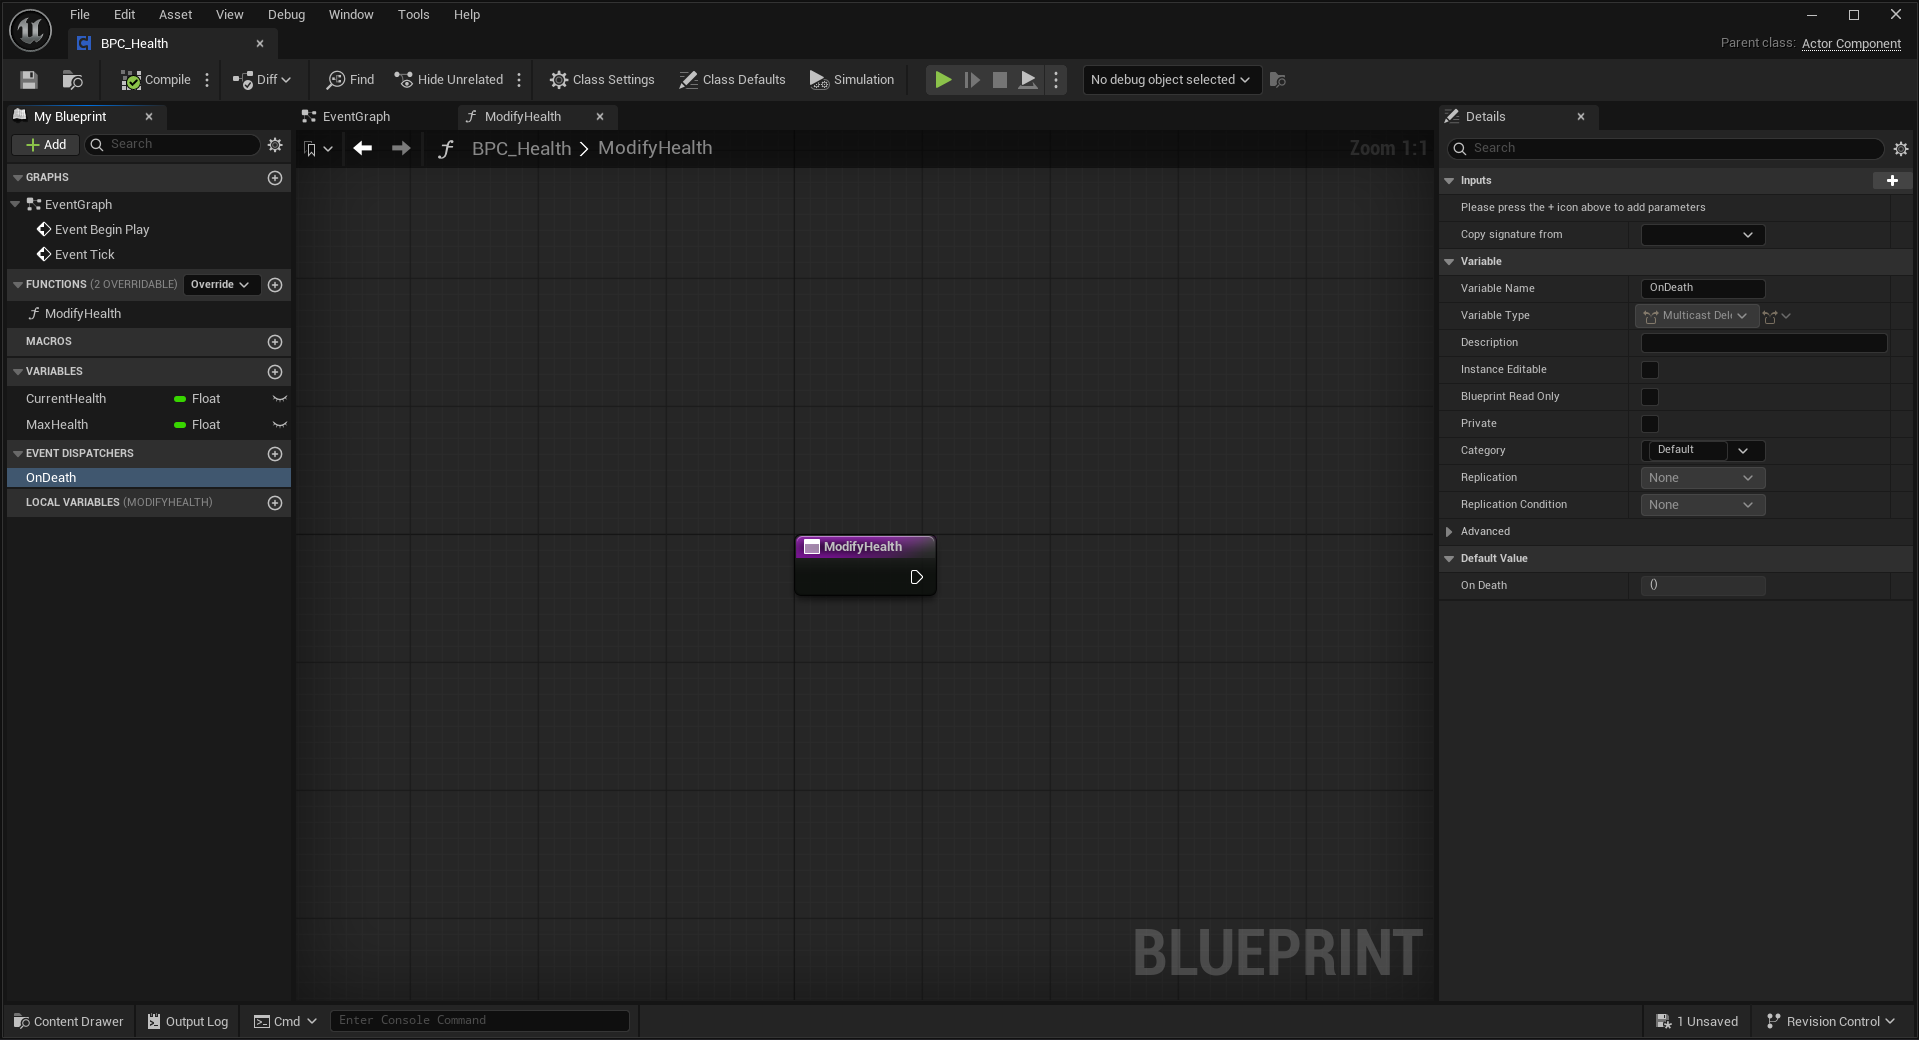
\includegraphics[width=0.9\textwidth]{images/ss-01-create-bpc-health.png}}
    \caption{Pembuatan Actor Component BPC\_Health beserta konfigurasi variabel, fungsi, dan event dispatcher.}
    \label{fig:ss-create-bpc}
\end{figure}

    \item \textbf{Inisialisasi nilai kesehatan pada BeginPlay.} Di tab Event Graph milik \texttt{BPC\_Health}, node \textbf{Event BeginPlay} dihubungkan ke node \textbf{SET CurrentHealth}. Nilai input SET disambungkan ke variabel \textbf{MaxHealth} supaya saat permainan dimulai, kesehatan karakter otomatis terisi penuh sesuai batas maksimal.

\begin{figure}[H]
    \centering
    \customfbox{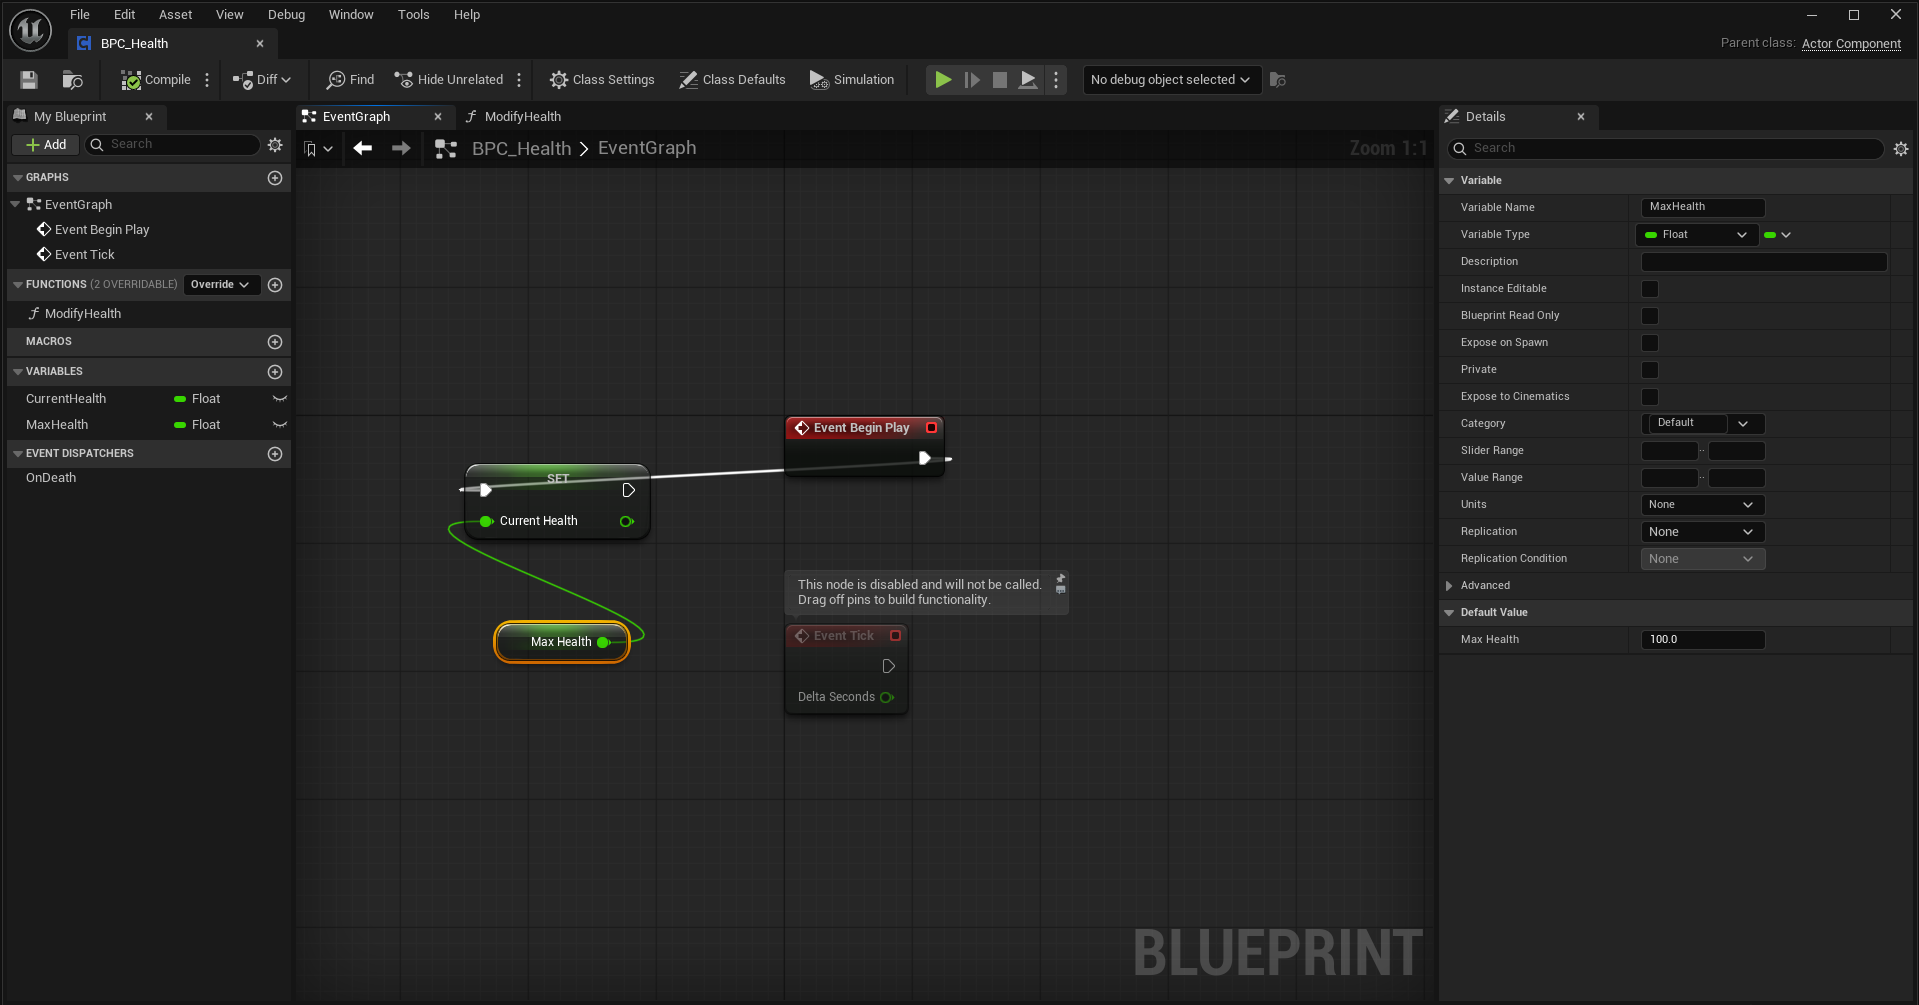
\includegraphics[width=0.9\textwidth]{images/ss-02-bpc-health-beginplay.png}}
    \caption{Event BeginPlay pada BPC\_Health yang mengisi CurrentHealth dari nilai MaxHealth.}
    \label{fig:ss-bpc-beginplay}
\end{figure}

    \item \textbf{Menyusun logika perhitungan fungsi ModifyHealth.} Fungsi \textbf{ModifyHealth} dibuka dan diberi parameter input float bernama \textbf{Health}. Logika graph disusun dengan mengurangkan \textbf{CurrentHealth} dengan nilai input tersebut. Hasil pengurangan dicek menggunakan node Branch pertama, disimpan kembali ke variabel \textbf{CurrentHealth}, lalu diperiksa lagi dengan node Branch kedua untuk kondisi nilai kurang dari atau sama dengan nol (\texttt{<= 0.0}). Jika True, alur memanggil node \textbf{Call OnDeath}.

\begin{figure}[H]
    \centering
    \customfbox{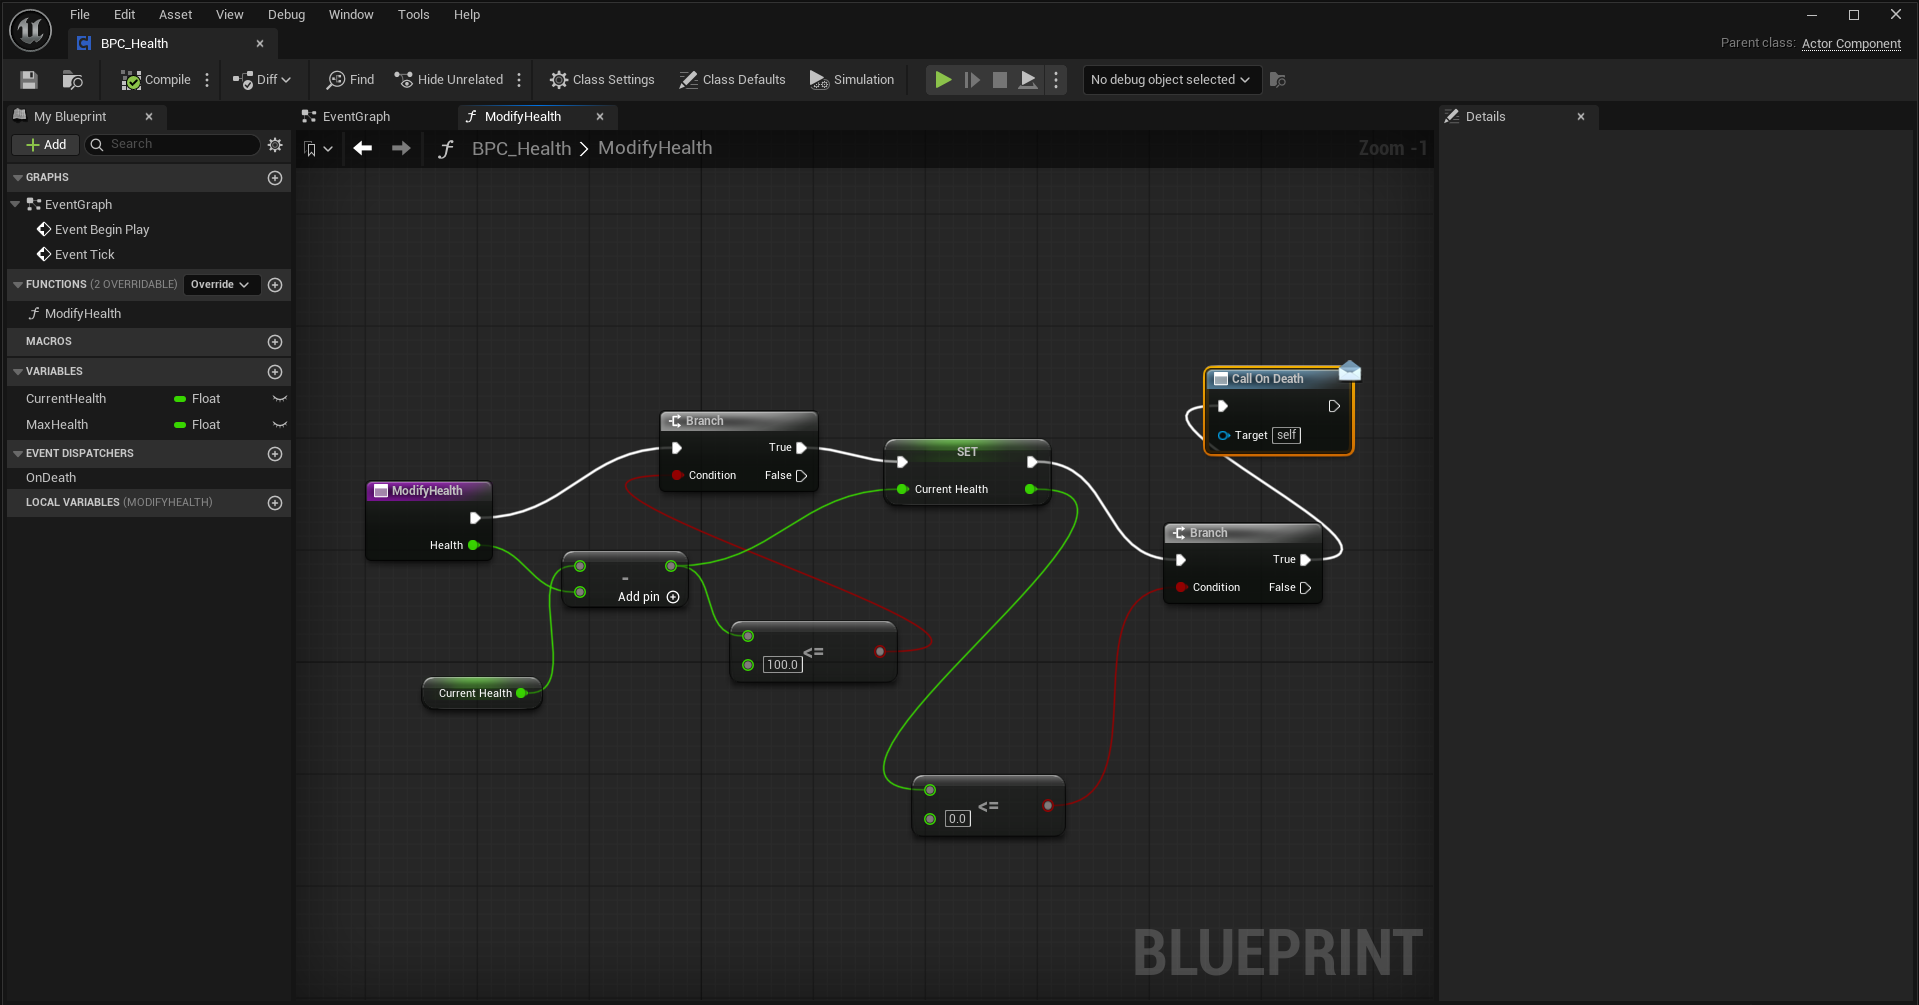
\includegraphics[width=0.9\textwidth]{images/ss-03-fungsi-modify-health.png}}
    \caption{Rangkaian graph fungsi ModifyHealth: kalkulasi pengurangan health dan pemanggilan Call OnDeath.}
    \label{fig:ss-modify-health}
\end{figure}

    \item \textbf{Memasang BPC\_Health ke BP\_ThirdPersonCharacter.} Karakter \texttt{BP\_ThirdPersonCharacter} dibuka pada Blueprint Editor. Komponen \textbf{BPC\_Health} diseret dari Content Drawer ke hierarki Components milik karakter, sehingga karakter memiliki modul pencatat kesehatannya sendiri.

\begin{figure}[H]
    \centering
    \customfbox{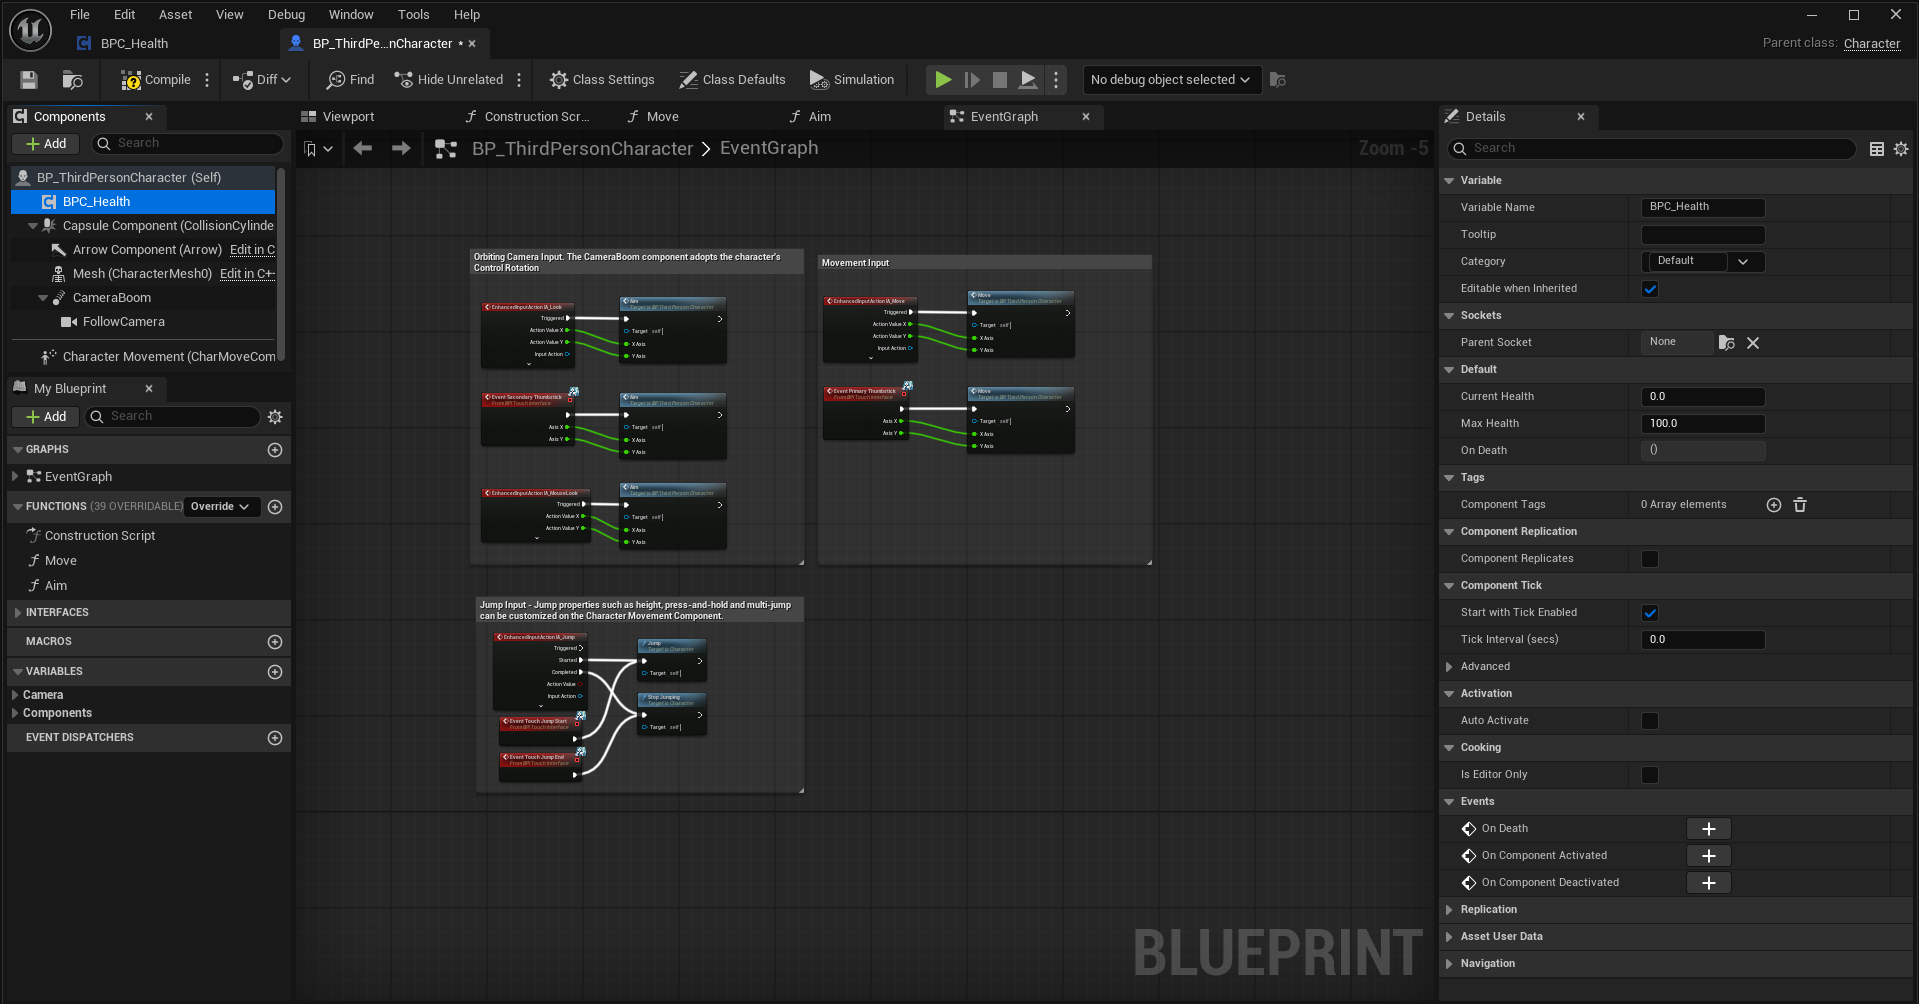
\includegraphics[width=0.9\textwidth]{images/ss-04-add-bpc-to-character.png}}
    \caption{Hierarki komponen BP\_ThirdPersonCharacter setelah penambahan komponen BPC\_Health.}
    \label{fig:ss-add-bpc}
\end{figure}

    \item \textbf{Binding Event OnDeath pada karakter.} Pada panel Components karakter, komponen \texttt{BPC\_Health} diklik kanan untuk menambahkan event \textbf{OnDeath}. Di Event Graph, node event ini dihubungkan ke node \textbf{Set Actor Scale 3D} dengan skala baru (0.0, 0.0, 0.0) dan target \textit{self}, sehingga karakter menyusut dan menghilang saat kehabisan darah.

\begin{figure}[H]
    \centering
    \customfbox{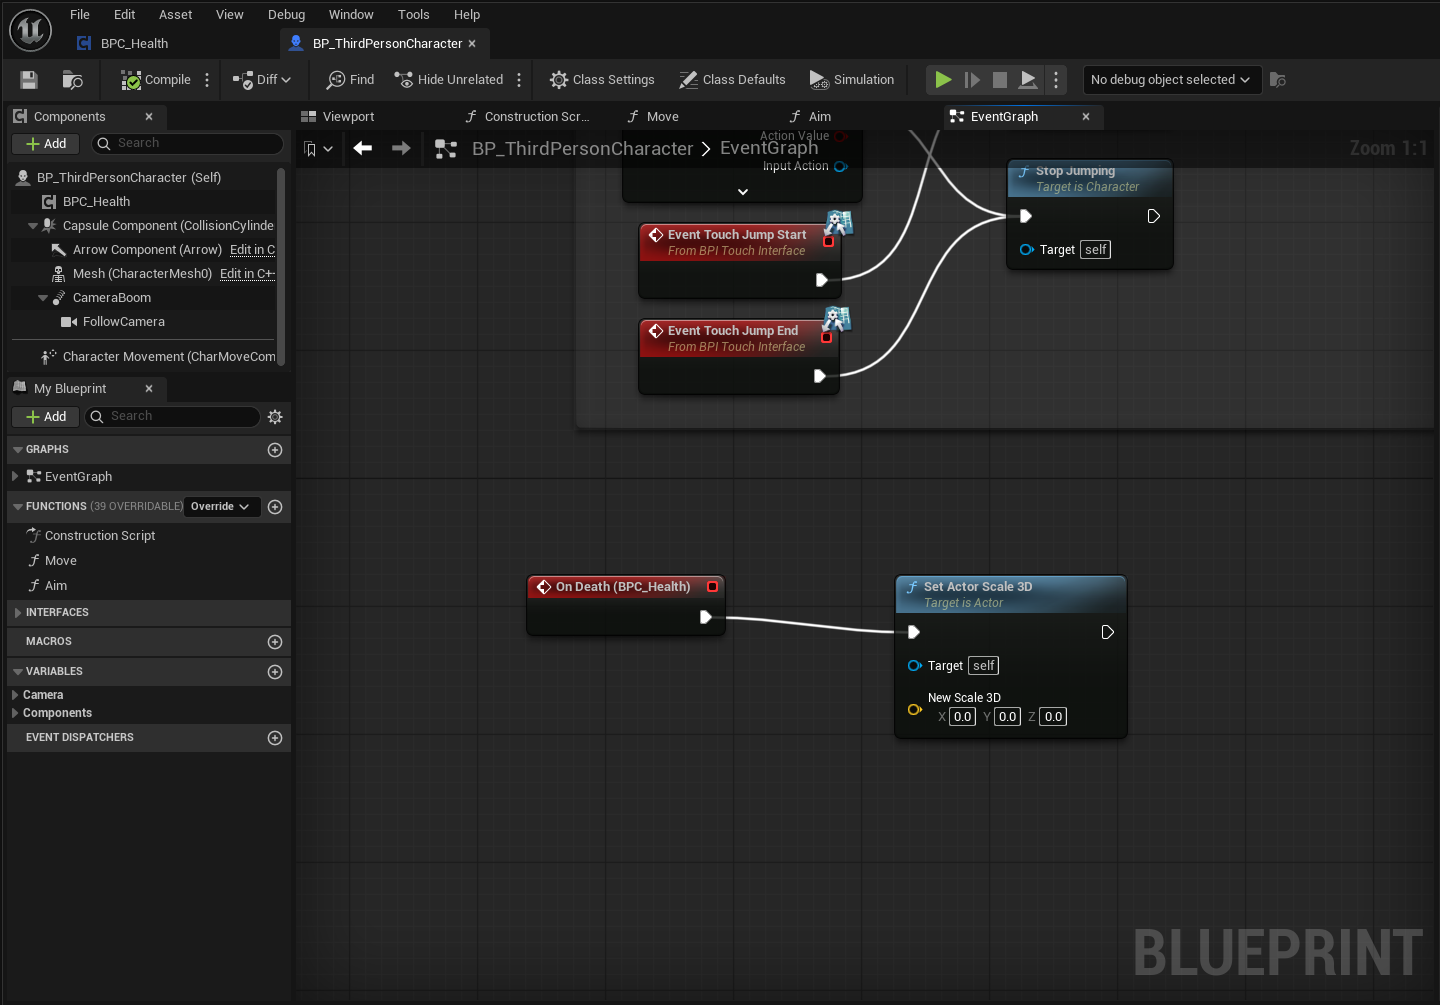
\includegraphics[width=0.9\textwidth]{images/ss-05-bind-ondeath-character.png}}
    \caption{Binding event OnDeath milik BPC\_Health pada BP\_ThirdPersonCharacter untuk mengubah skala karakter.}
    \label{fig:ss-bind-ondeath}
\end{figure}
\end{enumerate}

\subsection{Pembuatan dan Implementasi Blueprint Interface (BPI\_Overlap)}

\begin{enumerate}
    \item \textbf{Membuat folder Interfaces dan aset BPI\_Overlap.} Folder baru bernama \textbf{Interfaces} dibuat pada direktori utama konten. Di dalam folder ini, aset baru ditambahkan lewat klik kanan menu \textbf{Blueprint} lalu memilih \textbf{Blueprint Interface}. File dinamai \textbf{BPI\_Overlap} mengikuti aturan prefix standar.

\begin{figure}[H]
    \centering
    \customfbox{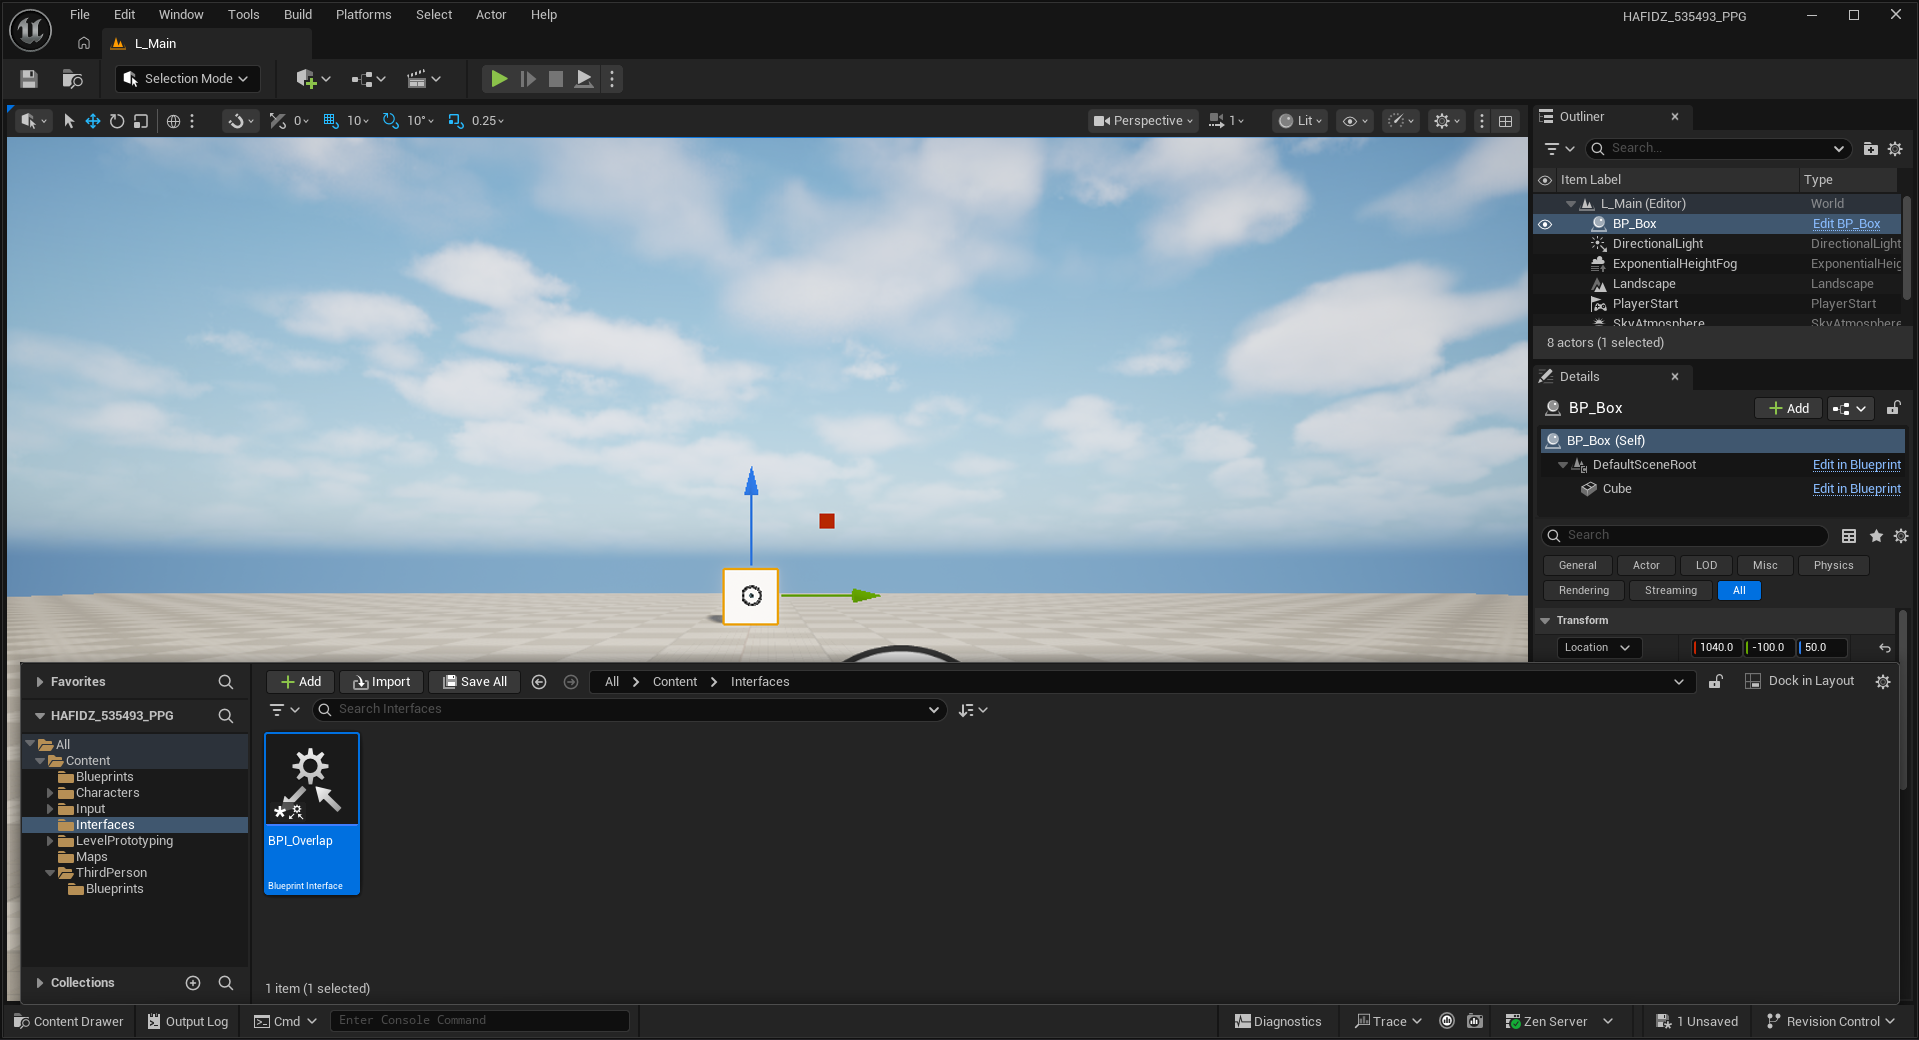
\includegraphics[width=0.9\textwidth]{images/ss-06-create-folder-interfaces.png}}
    \caption{Pembuatan folder Interfaces dan inisiasi aset Blueprint Interface BPI\_Overlap.}
    \label{fig:ss-create-bpi}
\end{figure}

    \item \textbf{Mendefinisikan fungsi TakeDamage pada Interface.} Aset \texttt{BPI\_Overlap} dibuka. Fungsi baru dibuat dan dinamai \textbf{TakeDamage}. Pada panel Details fungsi tersebut, sebuah parameter input bernama \textbf{AmountDamage} ditambahkan dengan tipe data Float.

\begin{figure}[H]
    \centering
    \customfbox{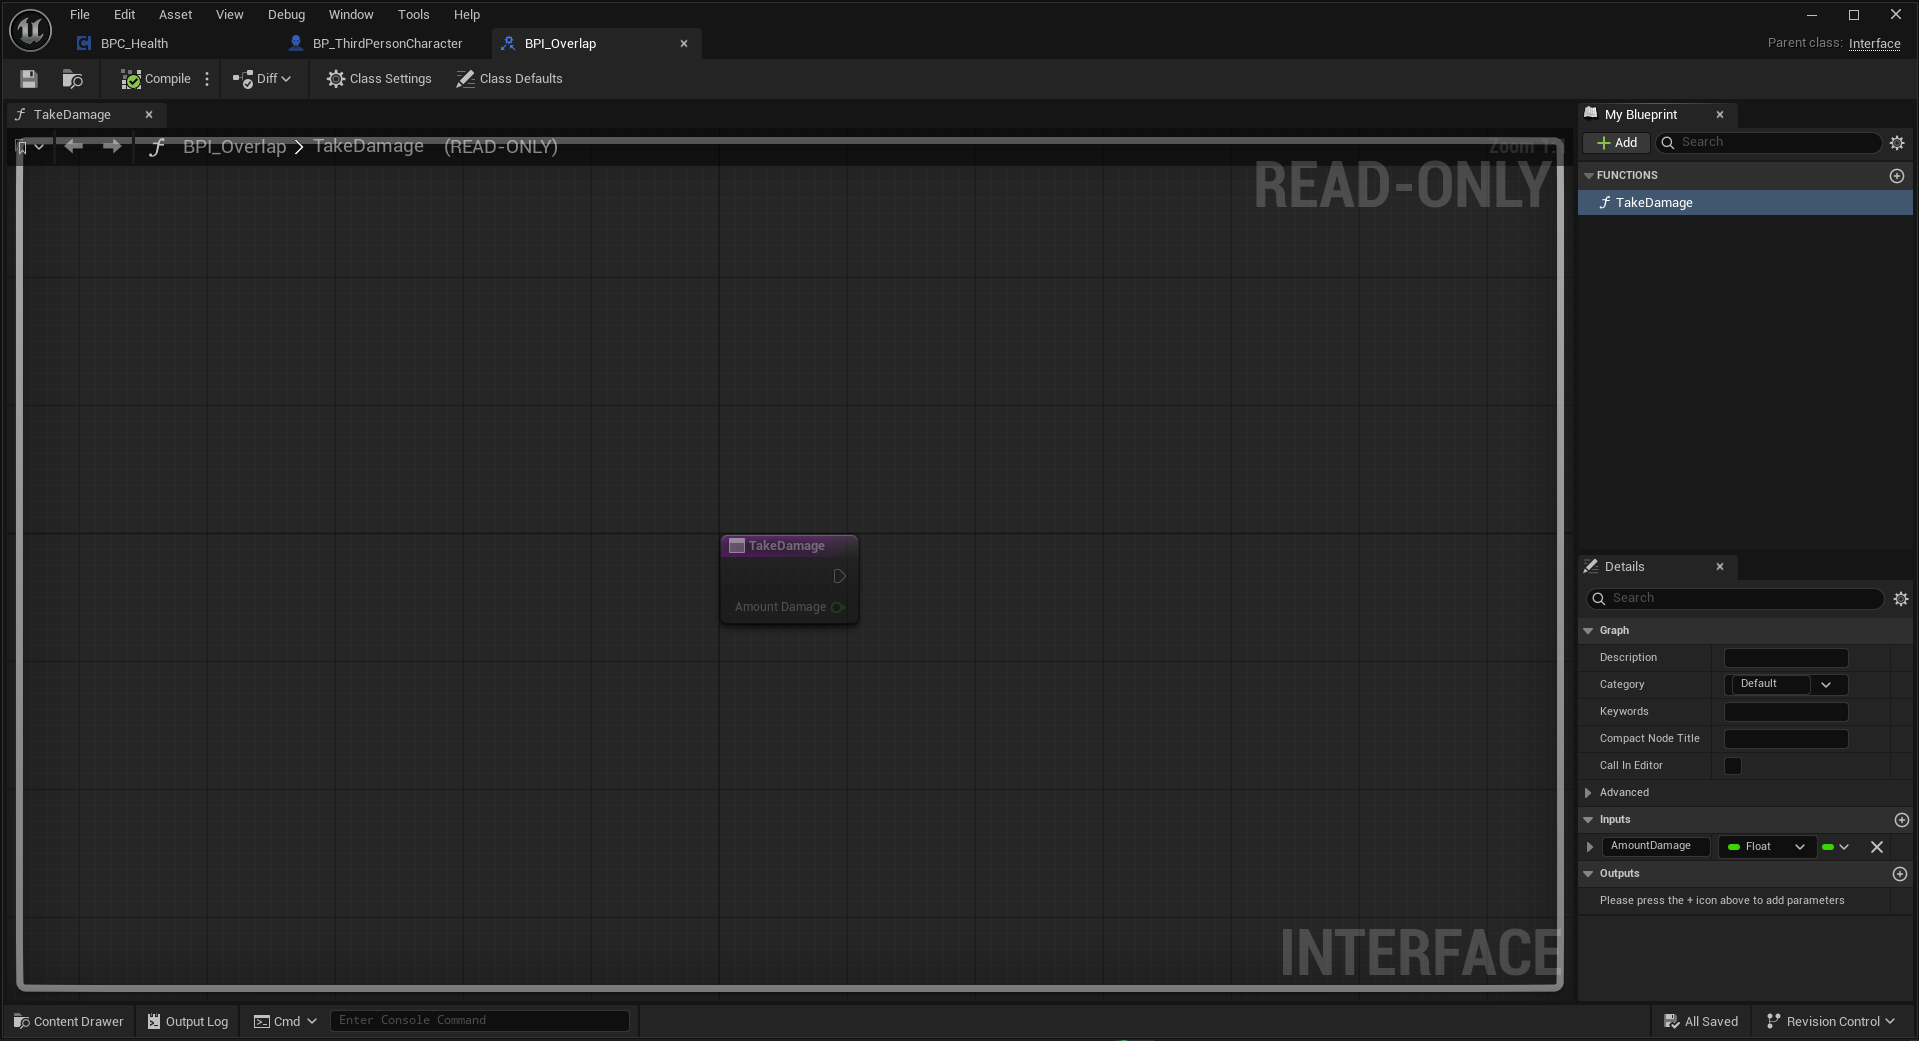
\includegraphics[width=0.9\textwidth]{images/ss-07-fungsi-take-damage.png}}
    \caption{Definisi fungsi TakeDamage dengan parameter masukan AmountDamage bertipe Float pada BPI\_Overlap.}
    \label{fig:ss-bpi-function}
\end{figure}

    \item \textbf{Mengimplementasikan Interface pada BP\_ThirdPersonCharacter.} Karakter \texttt{BP\_ThirdPersonCharacter} dibuka kembali. Pada toolbar atas, menu \textbf{Class Settings} diklik. Pada panel Details bagian \textbf{Interfaces > Implemented Interfaces}, tombol \textbf{Add} ditekan untuk memilih dan menambahkan interface \textbf{BPI\_Overlap}.

\begin{figure}[H]
    \centering
    \customfbox{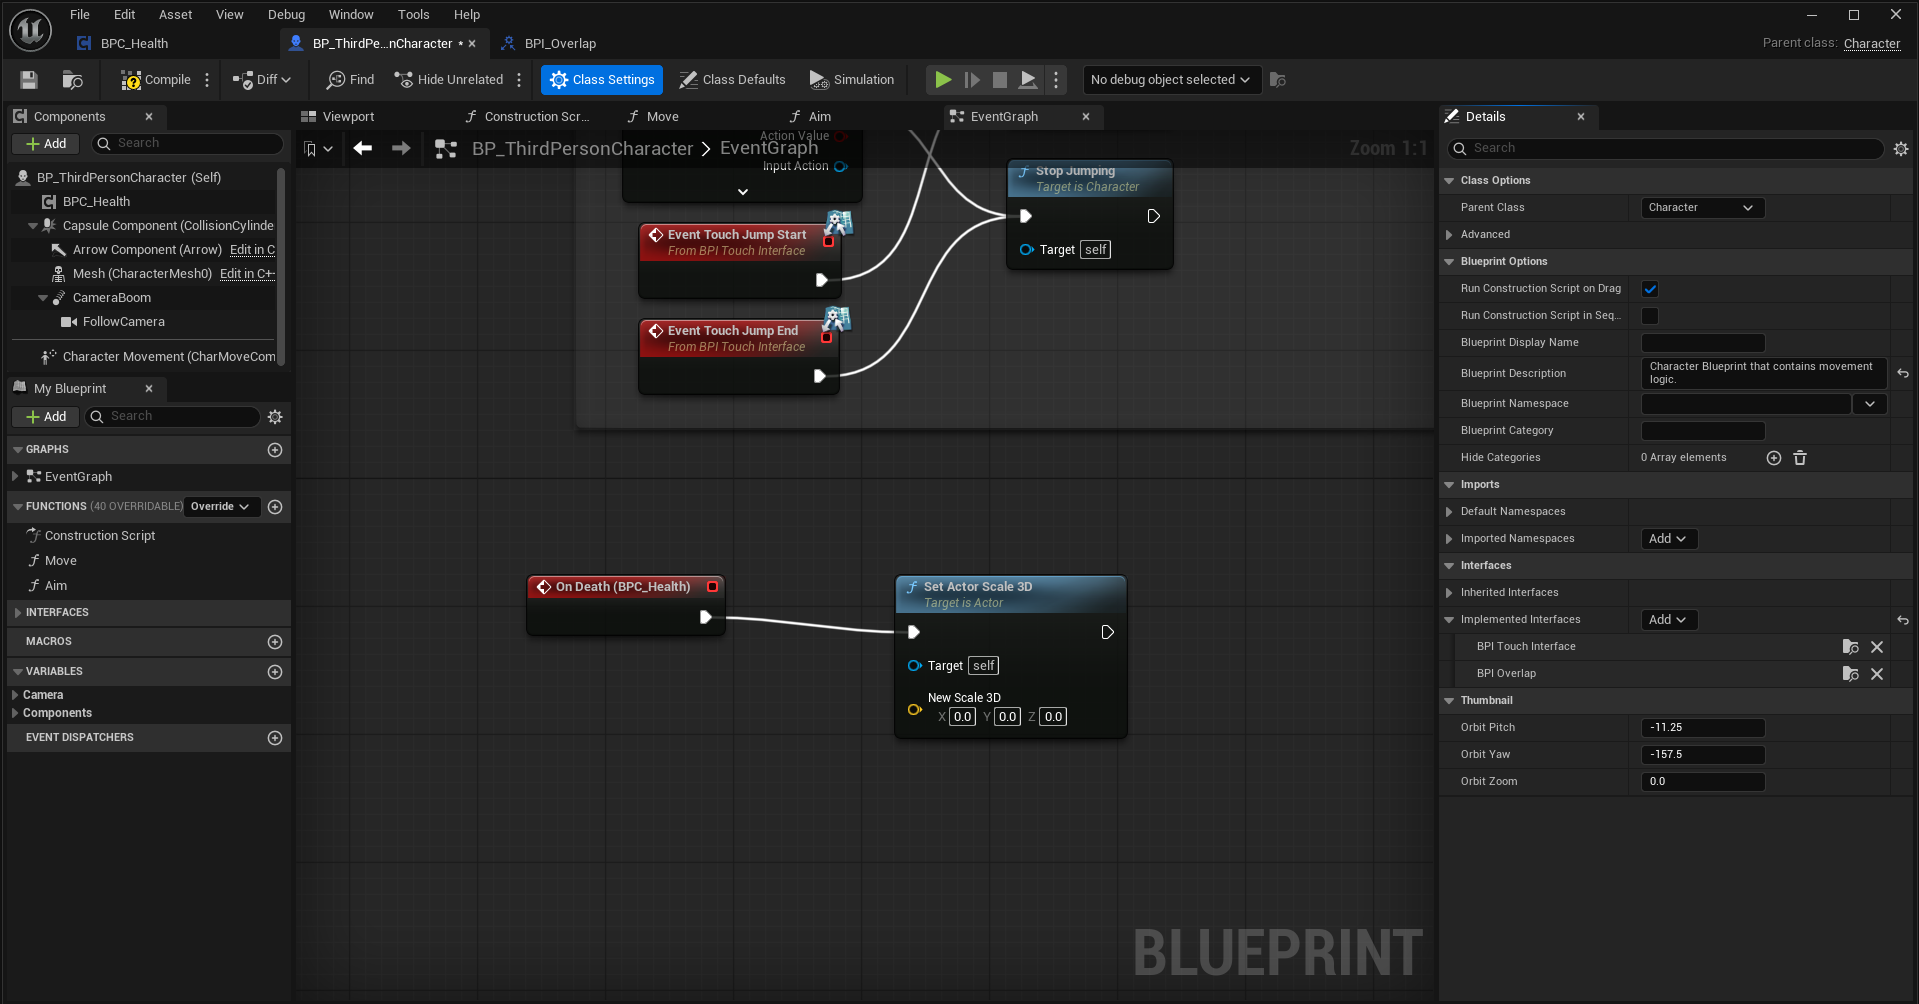
\includegraphics[width=0.9\textwidth]{images/ss-08-implement-interface-character.png}}
    \caption{Panel Class Settings BP\_ThirdPersonCharacter saat menambahkan BPI\_Overlap ke daftar antarmuka.}
    \label{fig:ss-impl-interface}
\end{figure}

    \item \textbf{Memeriksa fungsi Interface di panel My Blueprint.} Setelah Blueprint karakter dikompilasi, panel My Blueprint menampilkan kategori \textbf{Interfaces} yang memuat fungsi \textbf{TakeDamage}. Fungsi ini kini siap diimplementasikan sebagai event penanganan damage di Event Graph karakter.

\begin{figure}[H]
    \centering
    \customfbox{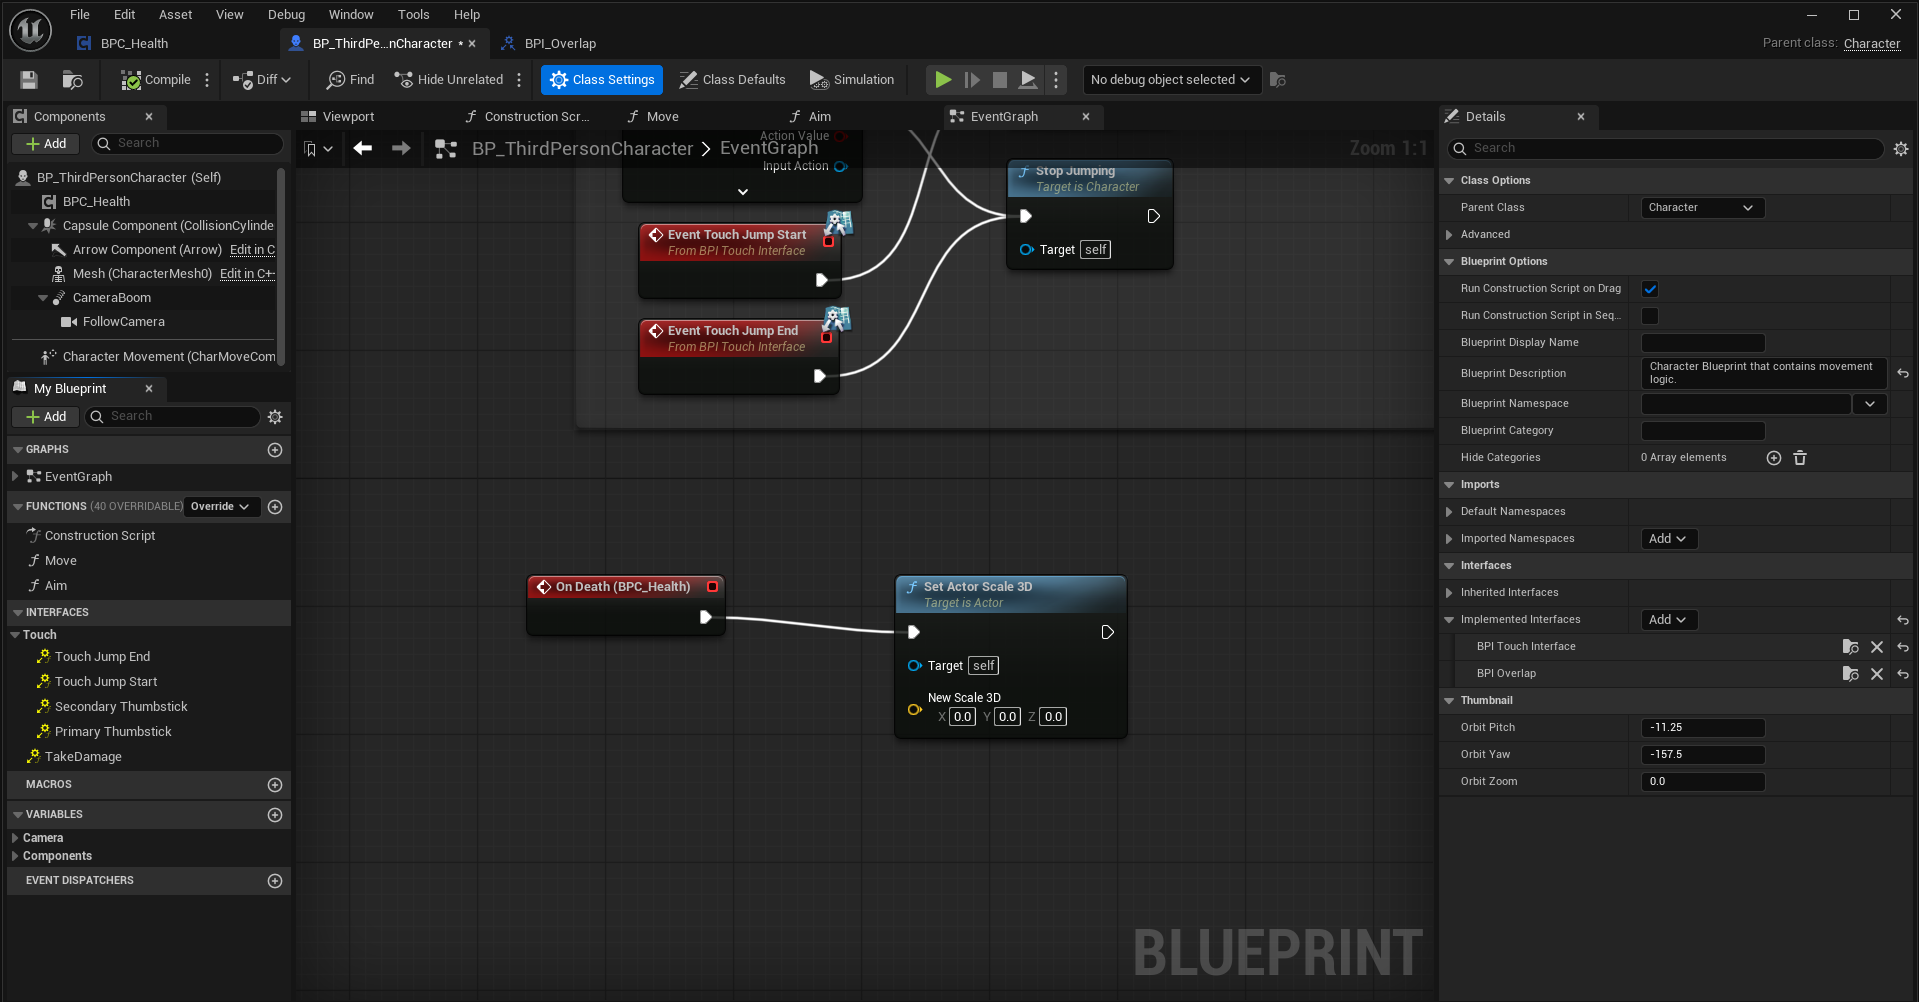
\includegraphics[width=0.9\textwidth]{images/ss-09-take-damage-in-myblueprint.png}}
    \caption{Kemunculan fungsi TakeDamage di bawah kategori Interfaces pada panel My Blueprint setelah kompilasi.}
    \label{fig:ss-myblueprint-interface}
\end{figure}

    \item \textbf{Menyusun logika Event TakeDamage pada karakter.} Fungsi \texttt{TakeDamage} dipasang ke Event Graph dengan klik kanan dan memilih \textit{Implement Event}. Node \textbf{Event TakeDamage} menerima nilai \textbf{AmountDamage}, lalu menyalurkannya ke pemanggilan fungsi \textbf{ModifyHealth} pada komponen \texttt{BPC\_Health}. Node \textbf{Print String} dengan teks \texttt{"Damage Taken!"} dipasang setelahnya untuk mencetak konfirmasi ke layar selama pengetesan.

\begin{figure}[H]
    \centering
    \customfbox{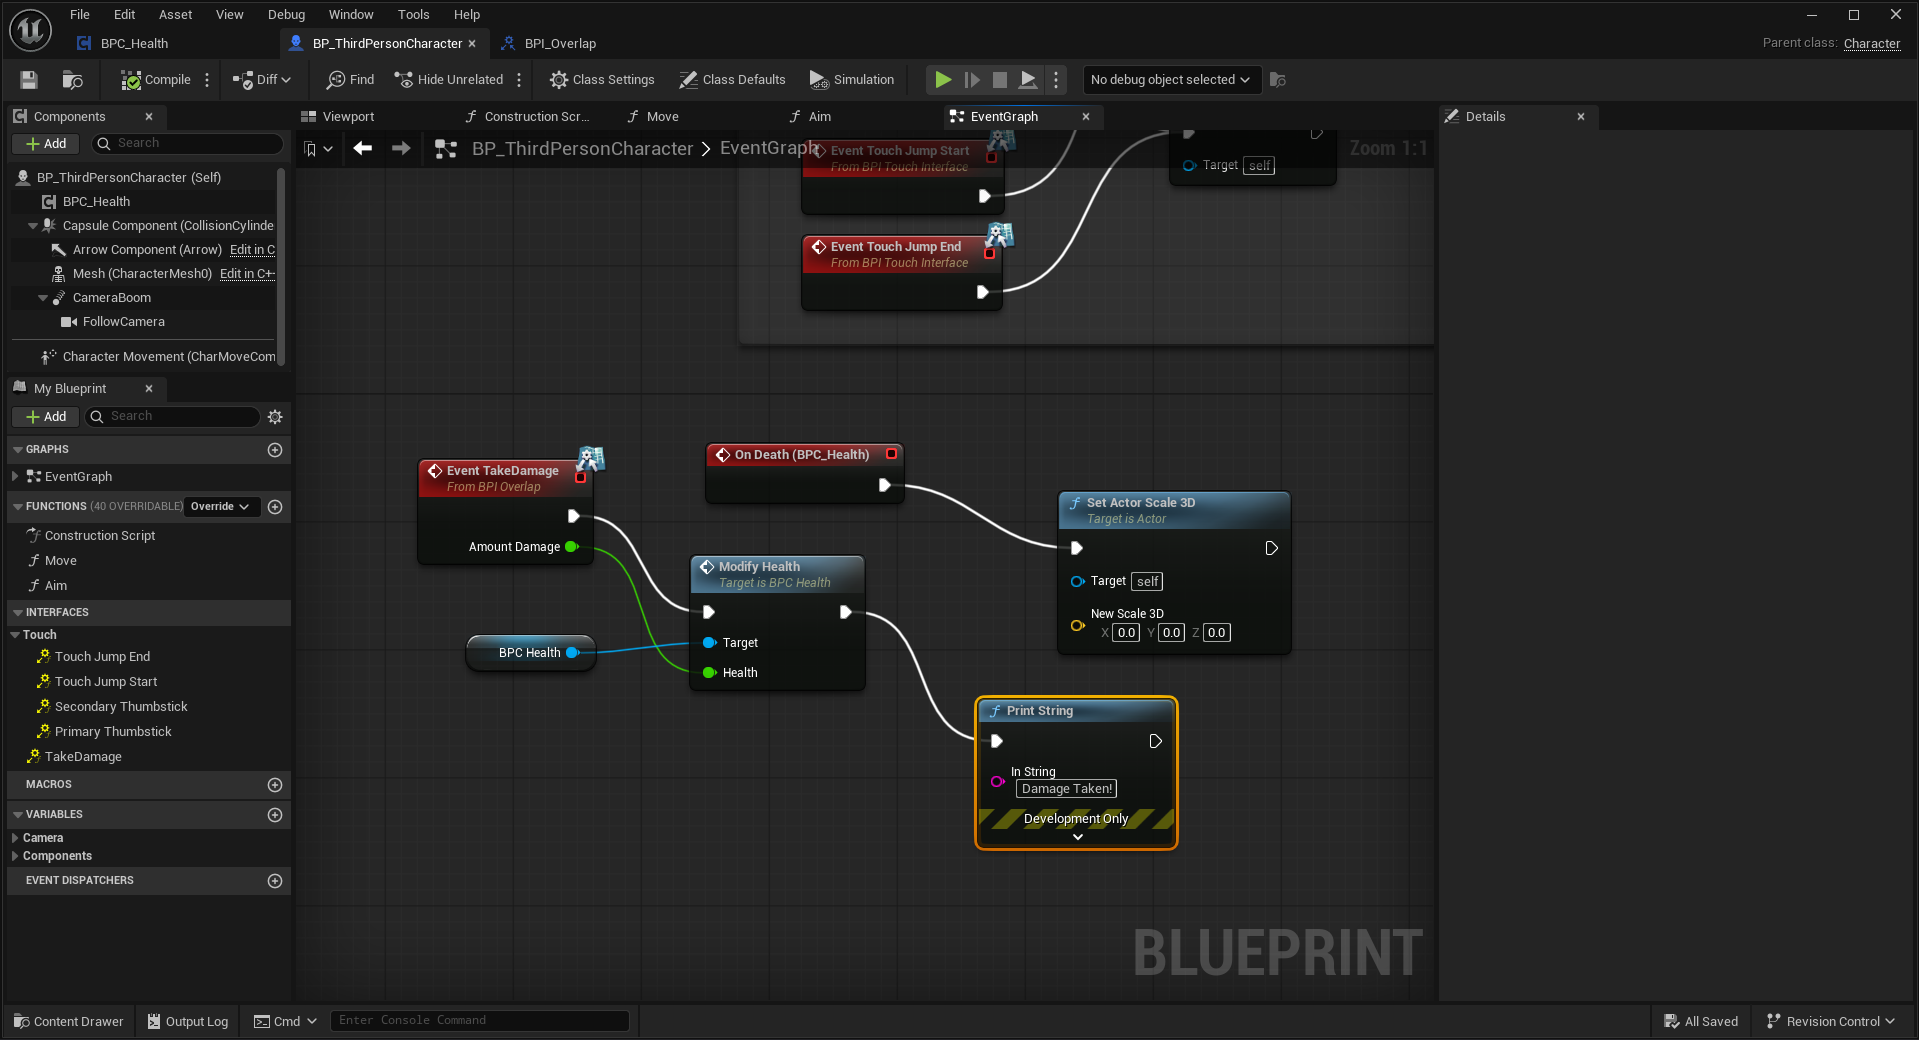
\includegraphics[width=0.9\textwidth]{images/ss-10-event-take-damage-character.png}}
    \caption{Implementasi Event TakeDamage di BP\_ThirdPersonCharacter terhubung ke fungsi ModifyHealth dan Print String.}
    \label{fig:ss-event-take-damage}
\end{figure}
\end{enumerate}

\subsection[Blueprint Actor Collision dan Parameter]{Blueprint Actor Collision dan Instance Editable Parameter (BP\_Collision)}

\begin{enumerate}
    \item \textbf{Membuat BP\_Collision dan merangkai OnComponentBeginOverlap.} Blueprint Actor baru dibuat dengan nama \textbf{BP\_Collision}. Di dalamnya ditambahkan komponen \textbf{Box Collision} dengan opsi \textit{Generate Overlap Events} aktif. Pada Event Graph, event \textbf{OnComponentBeginOverlap (Box)} dipasang dan pin \textbf{Other Actor} disambungkan ke panggilan pesan interface \textbf{TakeDamage (BPI Overlap)}.

\begin{figure}[H]
    \centering
    \customfbox{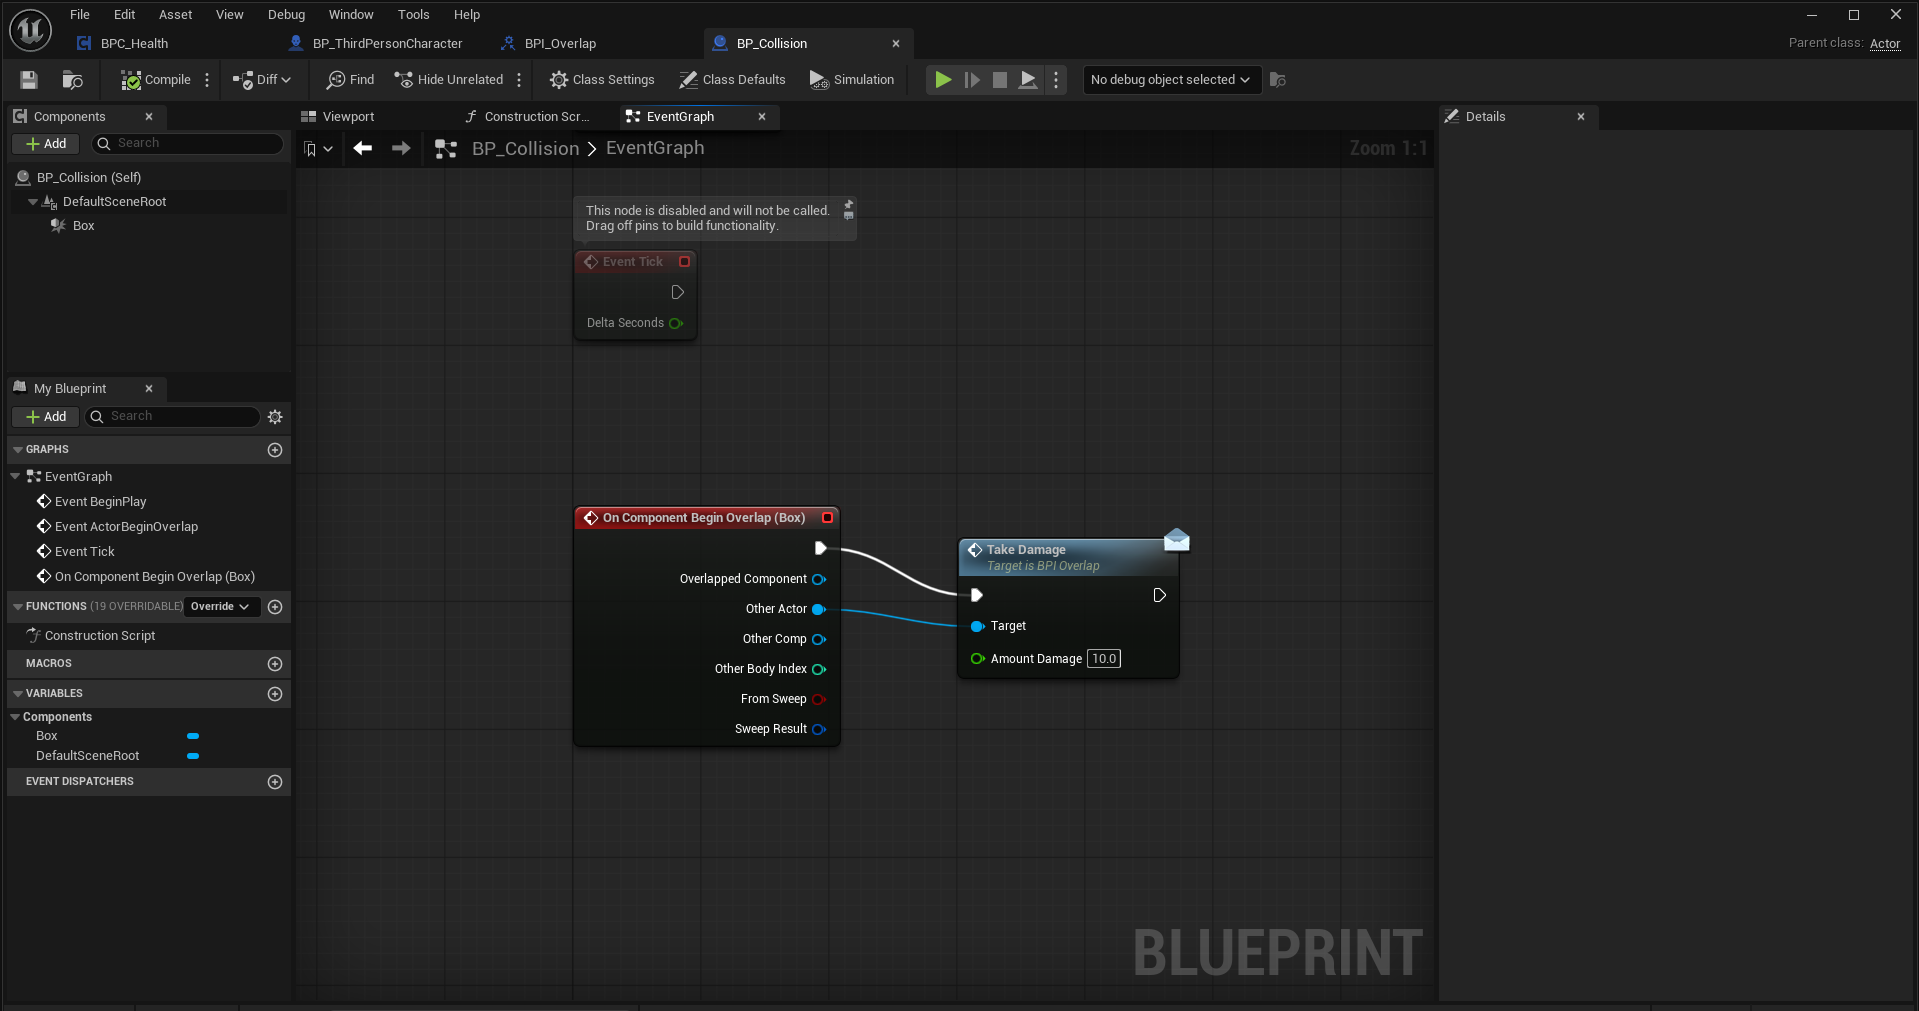
\includegraphics[width=0.9\textwidth]{images/ss-11-create-bp-collision.png}}
    \caption{Event Graph BP\_Collision: event OnComponentBeginOverlap memanggil fungsi interface TakeDamage.}
    \label{fig:ss-create-bp-collision}
\end{figure}

    \item \textbf{Menampilkan visual batas tabrakan di dalam game.} Komponen collision secara baku tidak terlihat saat game dimainkan. Agar batas kotak pemicu kelihatan saat pengujian, komponen \textbf{Box} dipilih pada panel Components \texttt{BP\_Collision}, lalu pada panel Details kategori \textbf{Rendering}, centang pada opsi \textbf{Hidden in Game} dimatikan.

\begin{figure}[H]
    \centering
    \customfbox{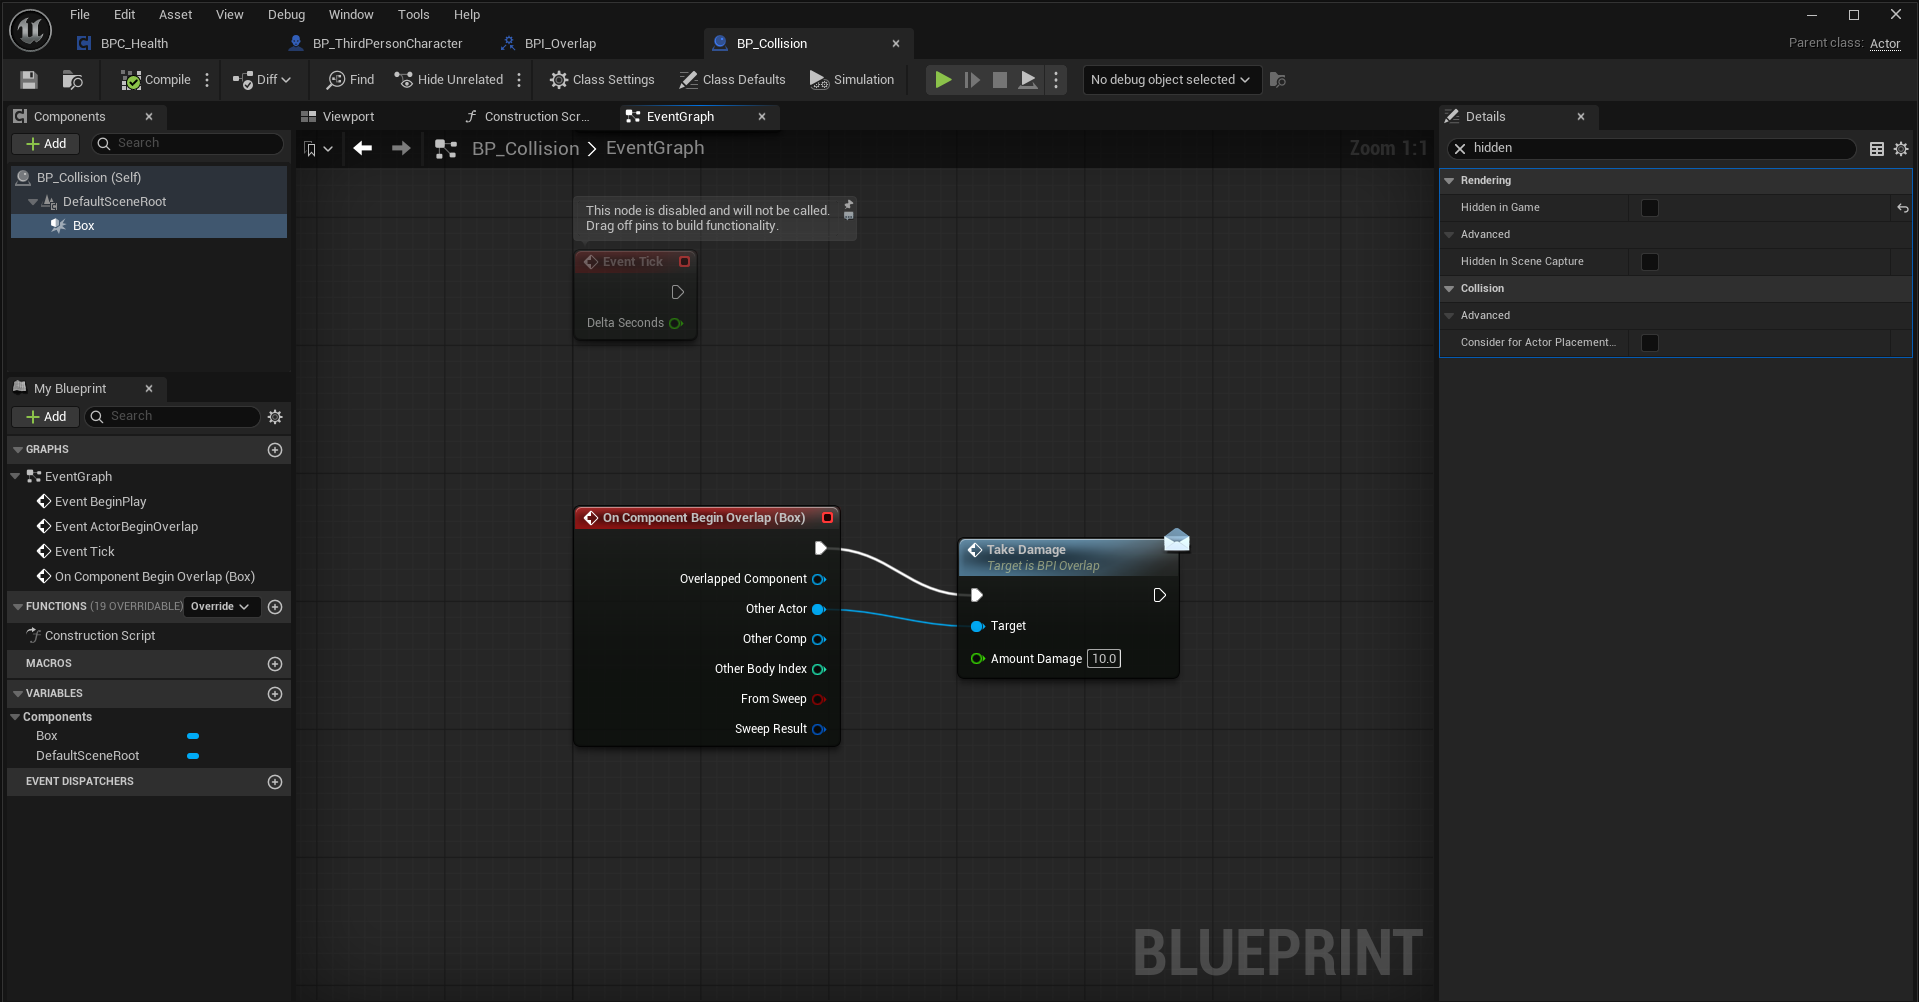
\includegraphics[width=0.9\textwidth]{images/ss-12-box-hidden-in-game.png}}
    \caption{Penonaktifan opsi Hidden in Game pada Box Collision agar batas pemicu terlihat saat simulasi.}
    \label{fig:ss-hidden-in-game}
\end{figure}

    \item \textbf{Menambahkan variabel Damage yang bersifat Instance Editable.} Pada panel My Blueprint \texttt{BP\_Collision}, variabel float baru bernama \textbf{Damage} dibuat dan opsi \textbf{Instance Editable} diaktifkan (ikon mata terbuka). Variabel ini disambungkan ke pin input \textbf{AmountDamage} pada node panggilan \texttt{TakeDamage}.

\begin{figure}[H]
    \centering
    \customfbox{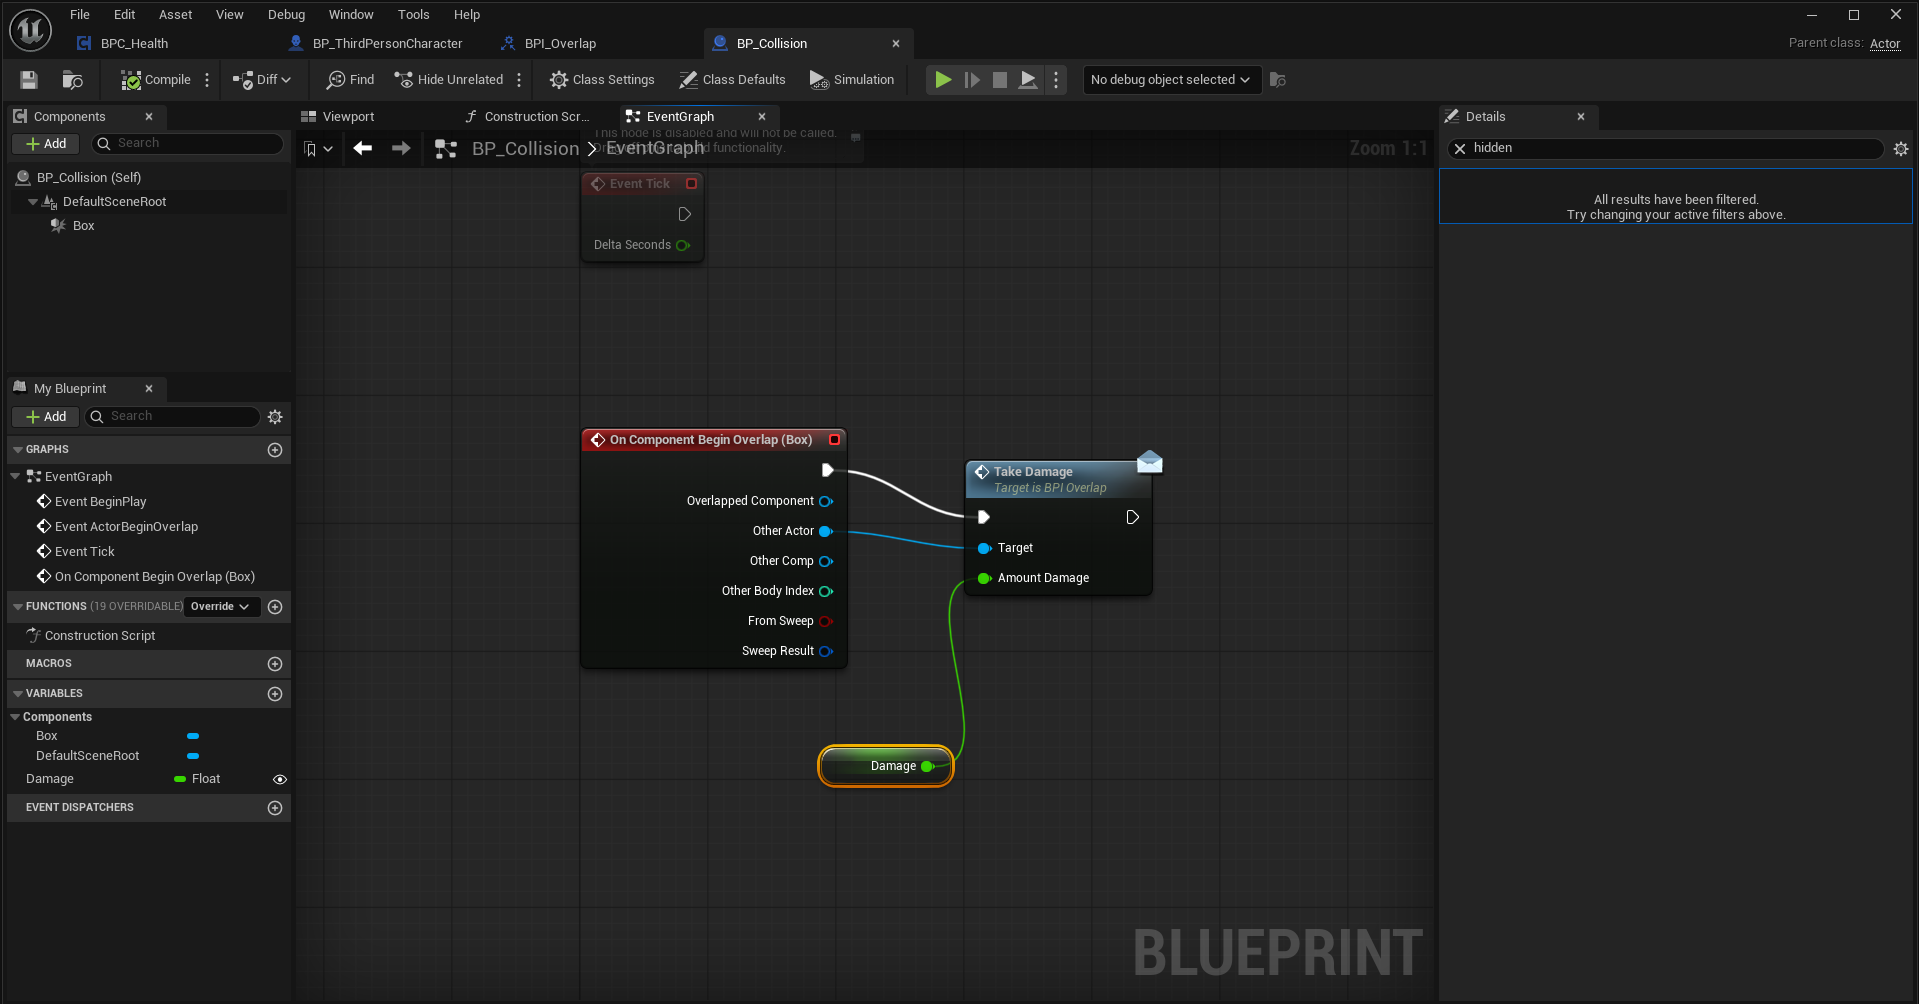
\includegraphics[width=0.9\textwidth]{images/ss-13-instance-editable-damage.png}}
    \caption{Variabel Damage dengan opsi Instance Editable terhubung ke pin masukan fungsi TakeDamage.}
    \label{fig:ss-instance-editable}
\end{figure}

    \item \textbf{Menempatkan instance BP\_Collision dan mengatur nilainya di Level.} Aktor \texttt{BP\_Collision} ditarik dari Content Drawer ke arena level. Pada panel Details instance aktor tersebut di level, nilai properti \textbf{Damage} diubah menjadi \textbf{30.0} langsung melalui editor level tanpa perlu membuka file Blueprint aslinya.

\begin{figure}[H]
    \centering
    \customfbox{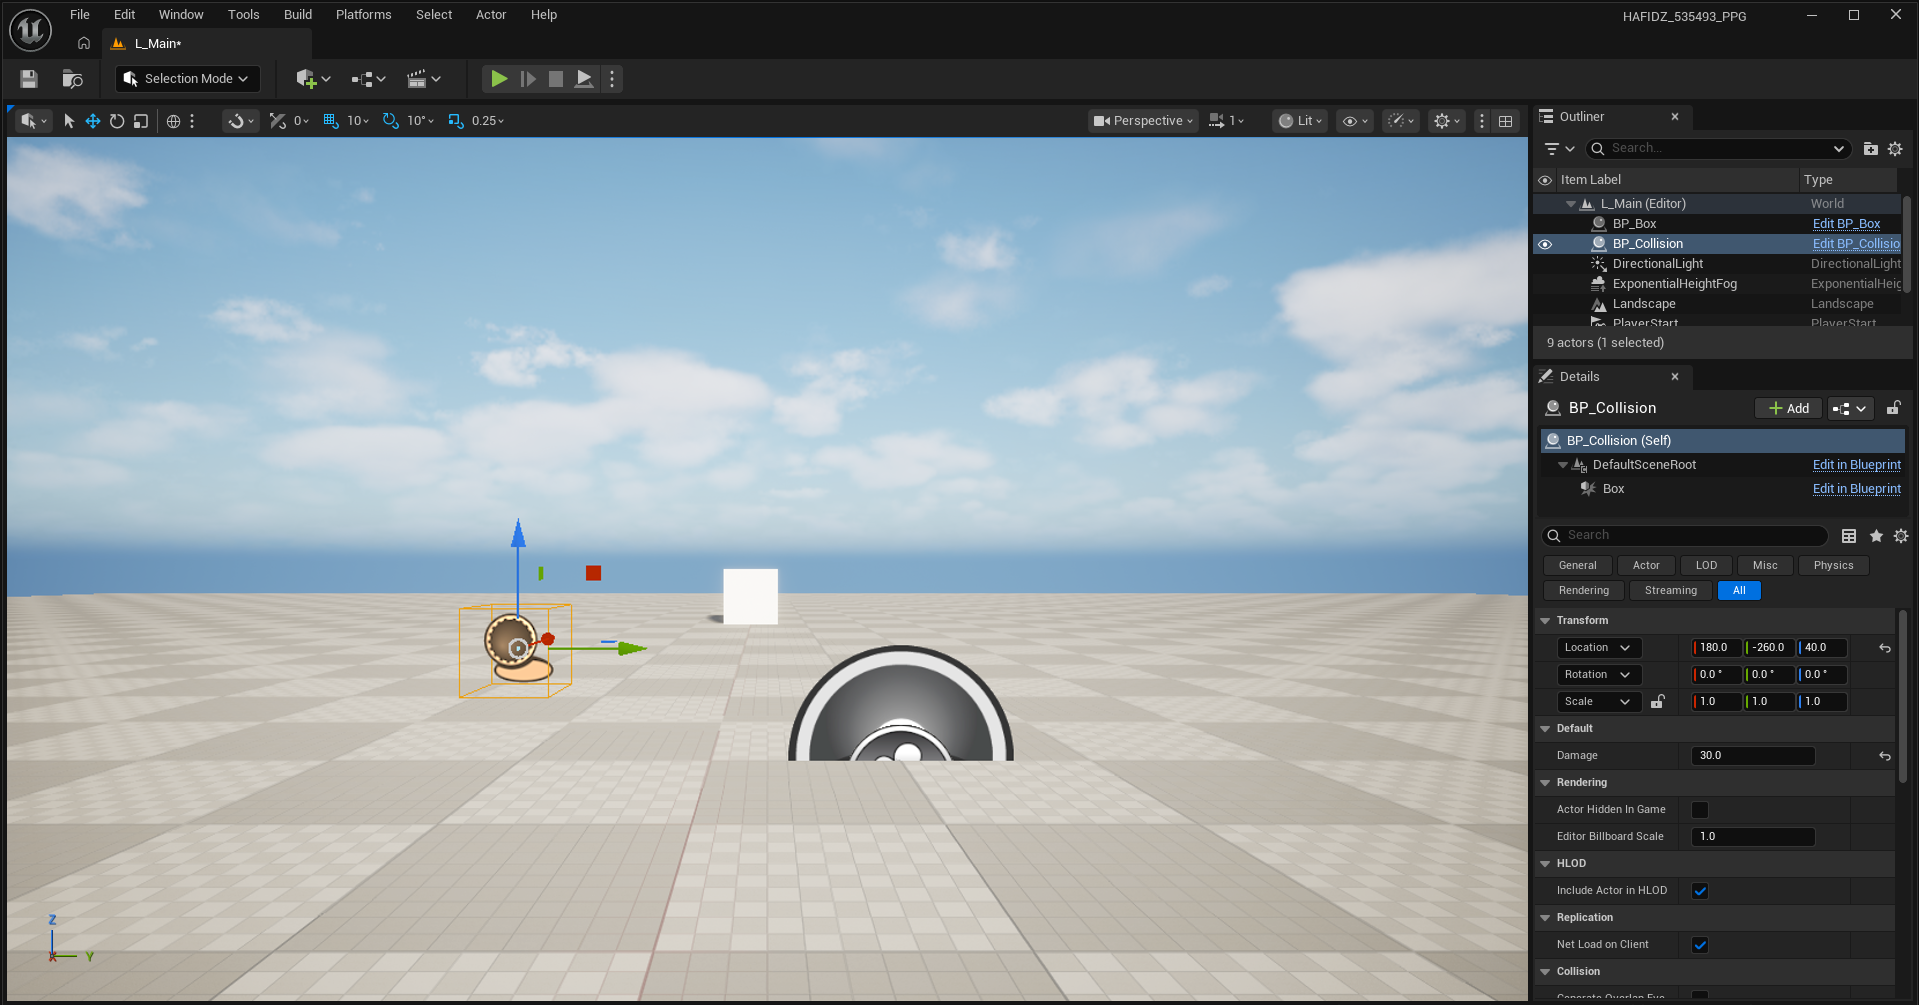
\includegraphics[width=0.9\textwidth]{images/ss-14-set-damage-in-level.png}}
    \caption{Pengubahan nilai parameter Damage menjadi 30.0 melalui panel Details instance BP\_Collision di level.}
    \label{fig:ss-level-damage-value}
\end{figure}
\end{enumerate}

\section{Hasil Akhir}
Rangkaian praktikum diuji langsung dengan menekan tombol Play pada editor level. Karakter Third Person digerakkan melintasi batas kawat pemicu \texttt{BP\_Collision}. Kontak tabrakan langsung memicu event overlap yang mengirimkan pesan interface \texttt{TakeDamage} tanpa memerlukan casting kelas secara langsung. Nilai damage sebesar 30.0 diproses oleh komponen \texttt{BPC\_Health} untuk mengurangi variabel kesehatan karakter, dan node Print String mencetak teks konfirmasi \texttt{"Damage Taken!"} di pojok kiri atas viewport di sela-sela log status tombol dari pengujian sebelumnya.

\begin{figure}[H]
    \centering
    \customfbox{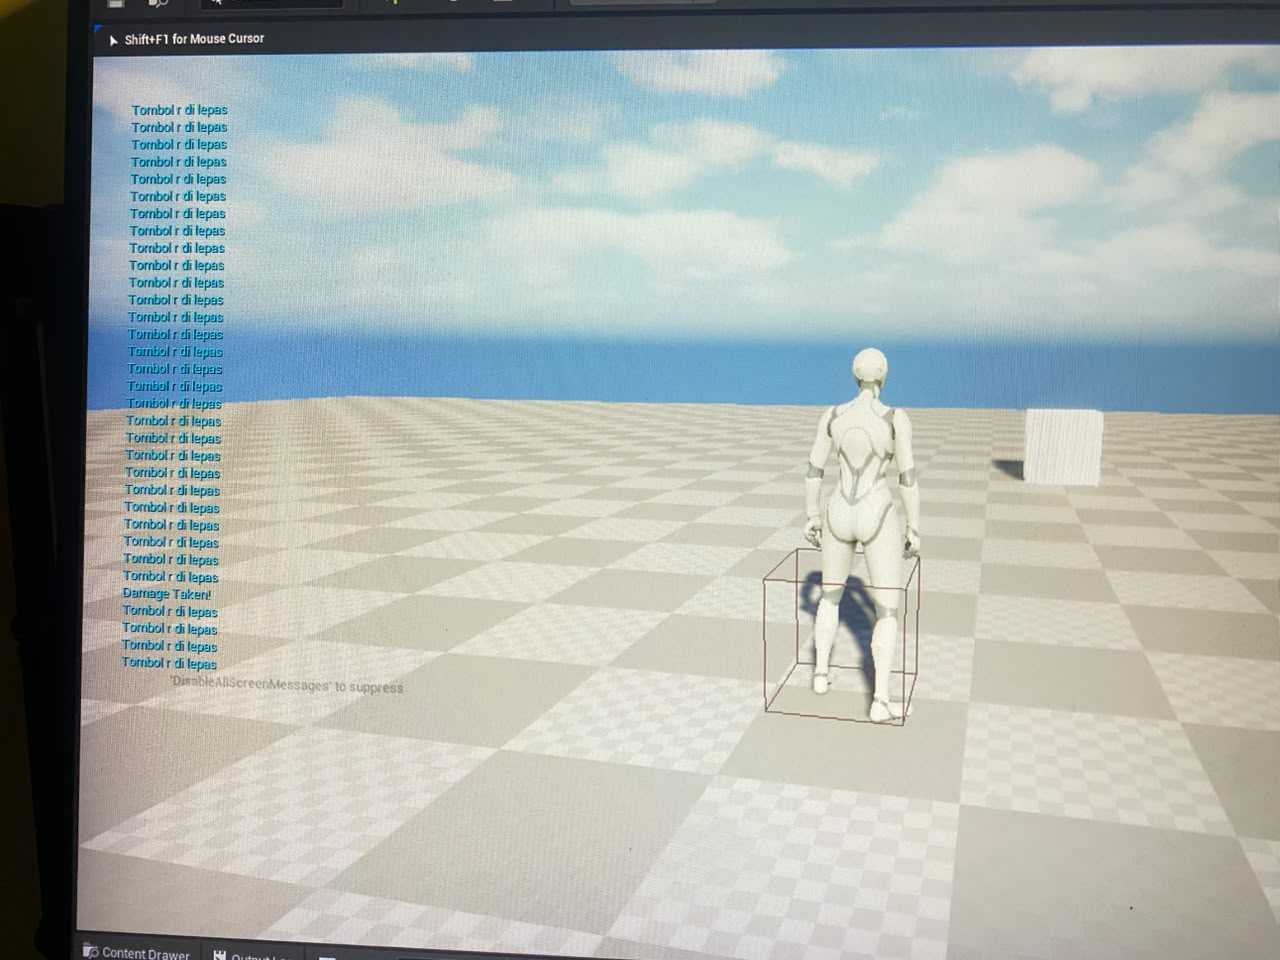
\includegraphics[width=0.9\textwidth]{images/ss-15-hasil-akhir-overlap-damage.png}}
    \caption{Karakter memasuki area Box Collision, memicu pesan interface TakeDamage dan mencetak teks debug Damage Taken!.}
    \label{fig:hasil-overlap}
\end{figure}

Pengujian dilanjutkan dengan mengarahkan karakter masuk ke dalam volume tabrakan berulang kali sampai akumulasi damage menghabiskan nilai kesehatan. Begitu nilai \texttt{CurrentHealth} menyentuh angka nol, fungsi \texttt{ModifyHealth} mengeksekusi pemanggilan event dispatcher \texttt{OnDeath}. Karakter \texttt{BP\_ThirdPersonCharacter} merespons event tersebut dengan menyetel skala tubuhnya ke (0.0, 0.0, 0.0). Karakter pun seketika lenyap dari pandangan, menyisakan kubus putih \texttt{BP\_Box} di latar belakang dan membuktikan seluruh alur logika telah terintegrasi penuh sesuai instruksi Modul 4 \cite{modul4}.

\begin{figure}[H]
    \centering
    \customfbox{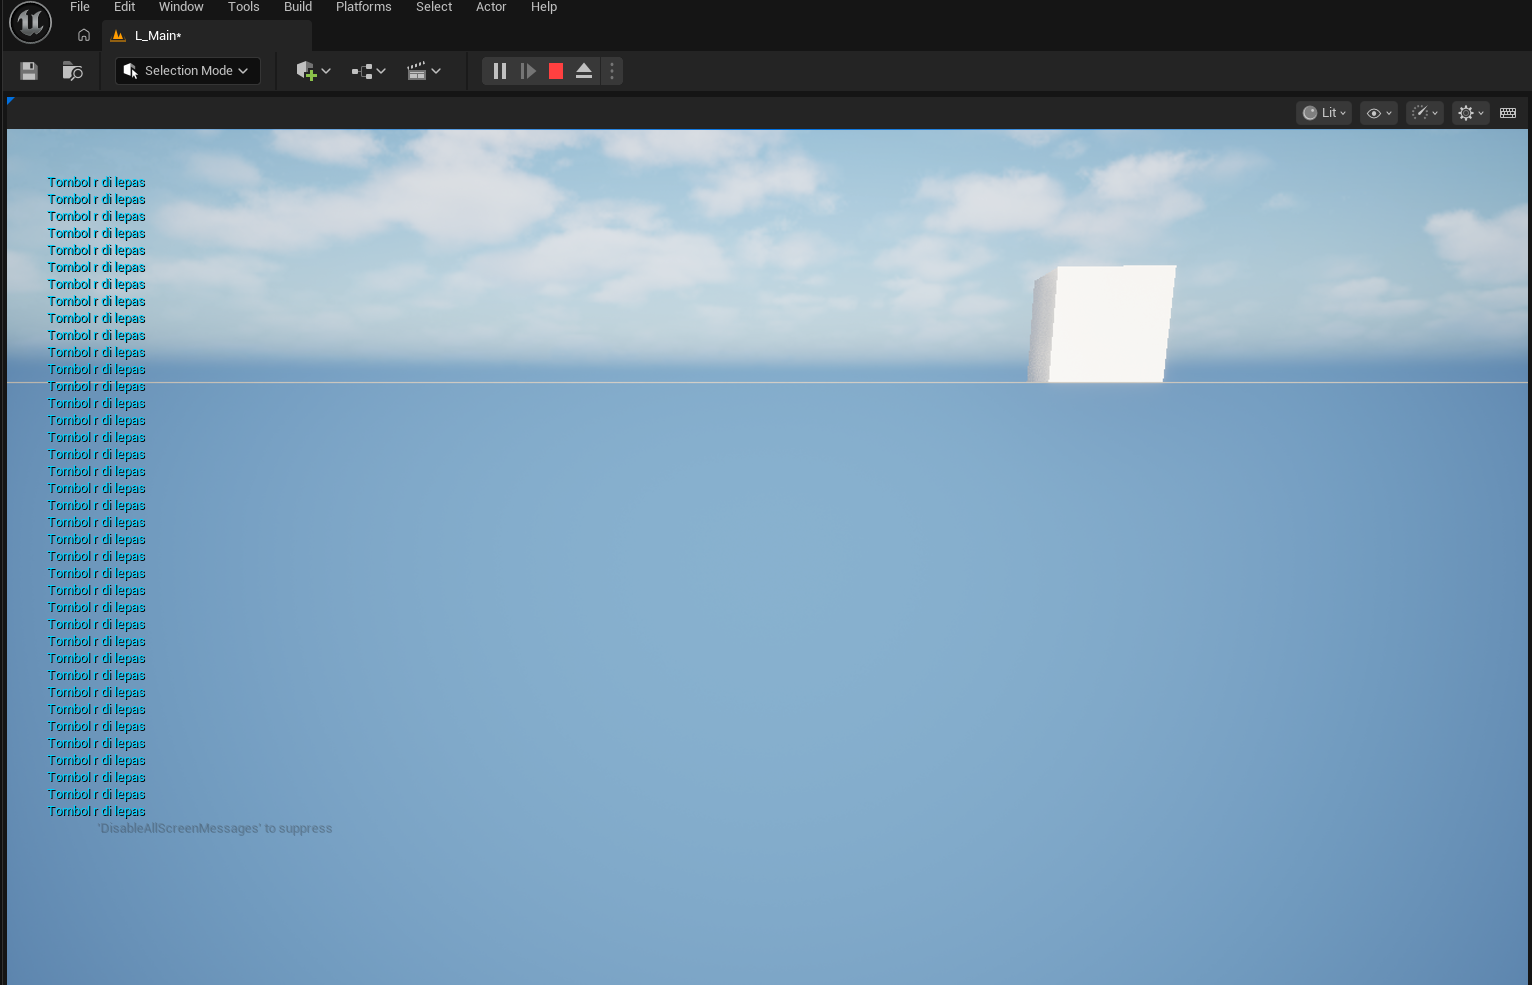
\includegraphics[width=0.9\textwidth]{images/ss-16-hasil-akhir-ondeath-scale.png}}
    \caption{Karakter kehabisan darah, memicu event dispatcher OnDeath dan melenyapkan karakter dengan skala nol.}
    \label{fig:hasil-ondeath}
\end{figure}

\clearpage

\chapter{Kesimpulan}
Dari praktikum Pertemuan 4 ini, saya memahami bahwa pemisahan logika menggunakan Actor Component membuat struktur Blueprint jauh lebih teratur. Komponen kesehatan \texttt{BPC\_Health} dapat berdiri sendiri dan ditempelkan ke aktor mana pun tanpa bergantung pada susunan internal kelas karakter pemain.

Event Dispatcher \texttt{OnDeath} terbukti memisahkan pencatatan data kesehatan dari aksi visual kematian. Komponen kesehatan cukup menyiarkan sinyal, sedangkan karakter pemilik yang menentukan responsnya, seperti mengecilkan skala tubuh hingga nol. Sementara itu, Blueprint Interface \texttt{BPI\_Overlap} menjadi jalur komunikasi pesan damage yang aman dan bersih tanpa memerlukan casting langsung (Cast to Class).

Terakhir, pemanfaatan Box Collision pada aktor \texttt{BP\_Collision} dengan variabel Instance Editable memberi kemudahan saat mendesain level. Nilai damage dapat disesuaikan per objek langsung dari panel Details di level tanpa menyentuh file Blueprint asal. Pola desain modular ini menjadi bekal yang rapi untuk membangun mekanisme gameplay yang lebih kompleks pada pertemuan berikutnya.

\clearpage
\addcontentsline{toc}{chapter}{Daftar Pustaka}
\renewcommand{\bibname}{Daftar Pustaka}
\begin{thebibliography}{99}
    \bibitem{modul4} Modul Praktikum Pengembangan Game Pertemuan 4: Interface, Component \& Collision, T.A. 2026/2027. Semester Gasal, Universitas Gadjah Mada.
    \bibitem{epic-components} Epic Games, ``Components in Unreal Engine'', 2026. [Online]. Tersedia: \url{https://dev.epicgames.com/documentation/en-us/unreal-engine/components-in-unreal-engine}.
    \bibitem{epic-dispatchers} Epic Games, ``Event Dispatchers in Unreal Engine'', 2026. [Online]. Tersedia: \url{https://dev.epicgames.com/documentation/en-us/unreal-engine/event-dispatchers-in-unreal-engine}.
    \bibitem{epic-interface} Epic Games, ``Blueprint Interface in Unreal Engine'', 2026. [Online]. Tersedia: \url{https://dev.epicgames.com/documentation/en-us/unreal-engine/blueprint-interface-in-unreal-engine}.
    \bibitem{epic-collision} Epic Games, ``Collision in Unreal Engine'', 2026. [Online]. Tersedia: \url{https://dev.epicgames.com/documentation/en-us/unreal-engine/collision-in-unreal-engine}.
    \bibitem{epic-collision-responses} Epic Games, ``Collision Response Reference in Unreal Engine'', 2026. [Online]. Tersedia: \url{https://dev.epicgames.com/documentation/en-us/unreal-engine/collision-responses-in-unreal-engine}.
    \bibitem{epic-variables} Epic Games, ``Blueprint Variables in Unreal Engine'', 2026. [Online]. Tersedia: \url{https://dev.epicgames.com/documentation/en-us/unreal-engine/blueprint-variables-in-unreal-engine}.
    \bibitem{epic-actors} Epic Games, ``Actors in Unreal Engine'', 2026. [Online]. Tersedia: \url{https://dev.epicgames.com/documentation/en-us/unreal-engine/actors-in-unreal-engine}.
    \bibitem{epic-naming} Epic Games, ``Recommended Asset Naming Conventions in Unreal Engine Projects'', 2026. [Online]. Tersedia: \url{https://dev.epicgames.com/documentation/en-us/unreal-engine/recommended-asset-naming-conventions-in-unreal-engine-projects}.
    \bibitem{yt-tutorial} Ali Elzoheiry, ``Unreal Engine 5 Beginner Tutorial - Blueprints, Interfaces \& Components'', 2023. [Online Video]. Tersedia: \url{https://www.youtube.com/watch?v=EQfml2D9hwE}.
\end{thebibliography}

\end{document}
